\documentclass[a4paper, 12pt]{article}

%\documentclass[a4paper, 12pt]{article}
\usepackage[T2A]{fontenc}
\usepackage[utf8]{inputenc}
%\usepackage[left=1cm,right=1cm,top=1cm,bottom=1.5cm,bindingoffset=0cm]{geometry}
\usepackage{geometry}
\usepackage{setspace}
\usepackage{amsmath}
\usepackage{amssymb}
\usepackage{esint}
\usepackage{mathtools}
\usepackage[english,russian]{babel}
\usepackage{misccorr}                                    %точка после номера секции
\usepackage{graphicx}
%\usepackage{caption}                                     %подпись плавающих             обьектов            
\usepackage{ upgreek }                    
%\captionsetup{labelformat=default,labelsep=period,labelfont=bf}
\usepackage{indentfirst}                                 % Красная строка
\usepackage{float}                                       % можно использовать Н в плавающих обьектах
\usepackage[usenames,dvipsnames,svgnames,table]{xcolor}
\usepackage{lettrine}
\usepackage{fancybox,fancyhdr}
\usepackage{bigints}
\usepackage{verbatim}
\bibliographystyle{unsrt}

\usepackage{amsthm, amssymb}


\geometry{a4paper, left=20mm, right=10mm, top=20mm, bottom=20mm}

%\mathindent=1em 
%\sloppy 
\textwidth = 17 cm 
%\oddsidemargin = -0.5cm 
\topmargin = -2cm \textheight = 25cm 
\setcounter{page}{0}
\DeclareGraphicsExtensions{.pdf,.png,.jpg,.eps}
\bibliographystyle{plain}

\usepackage[T2A]{fontenc} % Поддержка русских букв
\usepackage[utf8]{inputenc} % Кодировка utf8
%\usepackage{pscyr} % Нормальные шрифты

\usepackage{xcolor}
\usepackage{hyperref}

\renewcommand{\v}[1]{\boldsymbol{#1}}

\newtheorem{utv}{Утверждение}
\newtheorem{thm}{Теорема}
\newtheorem{prf}{Доказательство}
\newtheorem{dfn}{Определение}
\newtheorem{consequence}{Следствие}


% Цвета для гиперссылок
\definecolor{linkcolor}{HTML}{4B0082} % цвет ссылок
\definecolor{urlcolor}{HTML}{799B03} % цвет гиперссылок

\hypersetup{pdfstartview=FitH,  linkcolor=linkcolor,urlcolor=urlcolor, colorlinks=true}

%\usepackage[
%backend=biber, 
%sorting=nyt,
%bibstyle=gost-authoryear,
%citestyle=gost-authoryear
%]{biblatex}
%\addbibresource{library}

\setcounter{tocdepth}{4} 

%\renewcommand{\thesection}{(\roman{section})}
%\renewcommand{\thesection}{\Roman{section}}

%\renewcommand{\thesubsection}{(\roman{subsection})}
\renewcommand{\thesubsection}{\arabic{section}.\arabic{subsection}}

% переименовываем  список литературы в "список используемой литературы"
\renewcommand\refname{СПИСОК ЛИТЕРАТУРЫ}
\usepackage{amsthm}

\theoremstyle{plain}
\newtheorem{lemma}{Лемма} 

\theoremstyle{plain}
\newtheorem{theorem}{Теорема} 

\theoremstyle{definition}
\newtheorem{definition}{Условие} 

\theoremstyle{remark}
\newtheorem{remark}{Замечание} 


\begin{document}

    % Титульная информация (можно вынести в отдельный файл, если она громоздкая)
    \title{Хаотическая динамика и трансверсальные гомоклинические структуры в окрестности резонанса 3:1 в плоской эллиптической ограниченной задаче трех тел}
    %\author{И.~О.~Фамилия}
    \date{\today}
    \maketitle


    \tableofcontents

    % Аннотация и ключевые слова
    %\begin{abstract}
    %    \input{sections/00_abstract} % Можно и тут написать, но лучше вынести
    %\end{abstract}
    %\keywords{ключевое слово1, ключевое слово2}

    % Начинаем включать основные разделы
    \section{Введение}
        \subsection{Ограниченная эллиптическая задача трех тел и пояс астероидов}
        В настоящей работе рассматривается плоская ограниченная эллиптическая задача трех тел в случае резонансного отношения периодов 3:1 малого тела и Юпитера. Данная задача является предельным вариантом общей задачи трех тел, исследованию которой посвящено большое число работ. Начиная с исследований Ньютона, Эйлера, Клеро, Даламбера, Лапласа, Лагранжа, Якоби, Коши, Пуанкаре, задача трех тел дала развитие не только анализу, но и многим другим разделам математатики. 

Рассмотрим движение трех тел с гравитационным взаимодействием в пространстве. Будем обозначать величины, связанные с различными телами, индексами $A,J,S$ (условно астероид, Юпитер, Солнце). Тогда уравнения движения принимают вид:
\begin{equation*}
 \begin{cases}
   m_S \v{\ddot{r_S}} = 
   \frac{G m_S m_J}{|\v{r_J-r_S}|^3} (\v{r_J-r_S})+
   \frac{G m_S m_A}{|\v{r_A-r_S}|^3} (\v{r_A-r_S}), 
   \\
   m_J \v{\ddot{r_J}} = 
   \frac{G m_J m_S}{|\v{r_S-r_J}|^3} (\v{r_S-r_J})+
   \frac{G m_J m_A}{|\v{r_A-r_J}|^3} (\v{r_A-r_J}),
   \\
   m_A \v{\ddot{r_A}} = 
   \frac{G m_A m_S}{|\v{r_S-r_A}|^3} (\v{r_S-r_A})+
   \frac{G m_A m_J}{|\v{r_J-r_A}|^3} (\v{r_J-r_A}),
 \end{cases}
\end{equation*}
где $m_{k}$ ($k\in \{A, J, S\}$) - масса $k$-го тела, $r_{k}$ - его радиус-вектор, $G$ - гравитационная постоянная. Поделив уравнения на массы, стоящие в левых частях равенств, можно заметить, что уравнения не теряют смысл и в пределе, когда одна или несколько масс обращаются в нуль.

Данная система является динамической системой с 9 степенями свободы. Однако, если предположить, что движение всех тел происходит в плоскости, то число степеней свободы системы уменьшается до 6, что заметно упрощает дальнейший анализ. При этом задача называется плоской задачей трех тел. Такое предположение является физически обоснованным, поскольку большое число наблюдаемых звездных систем могут считаться плоскими в том смысле, что один из их линейных рамеров много меньше двух других. Кроме того, из астрономических наблюдений известно, что, если астероид влетает в солнечную систему под большим углом, то он не задерживается в ней надолго.

Предположим, что массы тел удовлетворяют соотношению: 
$$m_A \ll m_J \ll m_S.$$ 

В таком случае, учитывая малость $m_A$, слагаемые, содержащие его в правой части, можно отбросить:
\begin{equation*}
 \begin{cases}
   \v{\ddot{r}_{S}} = 
   \frac{G m_J}{|\v{r_J-r_S}|^3} (\v{r_J-r_S}),
   \\
   \v{\ddot{r}_{J}} = 
   \frac{G m_S}{|\v{r_S-r_J}|^3} (\v{r_S-r_J}),
   \\
   \v{\ddot{r}_{A}} = 
   \frac{G m_S}{|\v{r_S-r_A}|^3} (\v{r_S-r_A})+
   \frac{G m_J}{|\v{r_J-r_A}|^3} (\v{r_J-r_A}).
 \end{cases}
\end{equation*}

Заметим, что первые два уравнения не зависят от характеристик астероида и, таким образом, описывают задачу Кеплера о движении двух тел под действием гравитационных сил. Как известно \cite{dub}, задача Кеплера интегрируема. С другой стороны, третье уравнение описывает движение астероида в гравитационном поле двух массивных тел. Такая задача называется ограниченной плоской задачей трех тел.

Перейдем в систему координат Якоби \cite{dub}, связанную с центром масс тел $S$ и $J$:
$$
\v{r} = \v{r_J}-\v{r_S},\quad
\v{\rho} = \frac{m_S}{m_J+m_S} \v{r} - \v{r_J} + \v{r_A},\quad
\v{r_c} = \v{r_J} - \frac{m_S}{m_J+m_S} \v{r}.
$$

Производя замену переменных и учитывая слагаемые, возникающие при переходе в неинерциальную систему отсчета, получаем:
\begin{equation*}
\begin{cases}
\v{\ddot{r_c}} = 0, \\
\v{\ddot{r}} = -\frac{G(m_S+m_J)}{r^3} \v{r},  \\
\v{\ddot{\rho}} = [\v{\rho} \times \frac{d \dot{\Omega}}{dt}]  + 2[\v{\dot{\rho}} \times \v{\Omega}] + [\v{\Omega} \times [\v{\rho} \times \v{\Omega}]] + \frac{1}{m_A} \frac{G m_A m_S}{|\v{r_S-r_A}|^3} (\v{r_S-r_A})+
   \frac{G m_A m_J}{|\v{r_J-r_A}|^3} (\v{r_J-r_A}),  
 \end{cases}
\end{equation*}
где
$$
\v{\Omega} = \frac{[\v{r_c} \times \v{\dot{r_c}}]}{r_c^2}.
$$

Масштабным преобразованием координат и переобозначением констант можно  добиться того, что параметры системы удовлетворяют следующим условиям:
$$
G = 1,\quad 
m_j = \nu,\quad 
m_s = 1 - \nu,\quad
|\v{\Omega}| = 1.
$$

Тогда уравнения движения, описывающие движение малого тела, имеют вид:
\begin{equation*}
 \begin{cases}
   \ddot{\rho_x}=+2 \dot{\rho_y} + \rho_x - \frac{\partial U}{\partial \rho_x}, \\
   \ddot{\rho_y}=-2 \dot{\rho_x} + \rho_y - \frac{\partial U}{\partial \rho_y},
 \end{cases}
\end{equation*}
$$U(r, \v{\rho}) = - \frac{1-\nu}{\sqrt{\big(\rho_x + \nu r \big)^2 + \rho_y^2}} - \frac{\nu}{\sqrt{\big(\rho_x - (1-  \nu ) r \big)^2 + \rho_y^2}}.$$
Полученная система уравнений является системой Лагранжа с лагранжианом:
$$L = \frac{\dot{\rho_x}^2 + \dot{\rho_y}^2}{2} + \frac{{\rho_x}^2 + {\rho_y}^2}{2} + \rho_x \dot{\rho_y} - \rho_y \dot{\rho_x} - U(r,\v{\rho}) .$$
Применяя к лагранжиану преобразование Лежандра и вводя переменные:
$$
x = \rho_x,\quad
y = \rho_y,\quad
p_x = \dot{x} - y,\quad
p_y = \dot{y} + x,
$$
получаем гамильтониан системы:
$$H = \frac{p_x^2 + p_y^2}{2} + p_xy - p_yx + U(r,\v{\rho}).$$

Потенциал в гамильтониане содержит параметр $r = |\v{r}|$ (расстояние между Солнцем и Юпитером), который определяется из уравнения:
$$\v{\ddot{r}} = -\frac{G(m_S+m_J)}{r^3} \v{r},$$
и в общем случае зависит от времени. Это уравнение является частным случаем задачи Кеплера, для которой известно точное решение. 

Известно, что эксцентриситет Юпитера достаточно мал (порядка $e_{J}\approx 0.05$), и потому его орбита близка к круговой. В пределе $e_{J}\to 0$ расстояние $r$ постоянно и мы получаем так называемую круговую плоскую ограниченную задачу трех тел. Данная задача описывается системой с двумя степенями свободы. Следует отметить, что круговая задача интегрируема, т.к. помимо интеграла энергии, она имеет второй интеграл движения - интеграл Якоби:
$$
\dot \rho_{x}^{2} + \dot \rho_{y}^{2} - \rho_{x}^{2} - \rho_{y}^{2} - 2 U(\rho_{x}, \rho_{y}) = {\rm const}.
$$

Однако, как показывают исследования \cite{fejoz, kaloshin}, учет эксцентриситета Юпитера $e_J$ является необходимым для рассмотрения хаотических процессов в системе. В предположении $e_{J}>0$ задача называется плоской эллиптической ограниченной задачей трех тел. 


        \subsection{Окрестность резонанса}
         
Для рассмотрения резонансного случая удобно перейти в систему координат Делоне, в которой гамильтониан имеет вид \cite{plummer}:
$$H = - \frac{(1-\nu)^2}{2L^2} - \nu R(L, \rho_1, \rho_2, l, \omega_1, \omega_2),$$
где возмущающая функция $R$ равна:
$$R = \sum_{s-j-k+p-m-n=0, s \geq 0} K^{sjkpmn}(L, \rho_1, \rho_2) \cos(s l + p l_J + j \omega_1 + k \omega_2 + m \omega_{1J} + n \omega_{2J}).$$
Здесь $(1-\nu)$ - масса Солнца, $\nu \approx \frac{1}{1000}$ - масса Юпитера, являющаяся малым параметром. Все углы, относящиеся к Юпитеру, обозначены индексом $J$, а углы, связанные с астероидом, обозначаются без индекса, гравитационная постоянная полагается равной единице. В терминах эллиптических элементов переменные выражаются формулами:
$$L = \sqrt{(1-\nu)a},$$
$$\rho_1 = \sqrt{(1-\nu)a}(1-\sqrt{1-e^2}),$$
$$\rho_2 = \sqrt{(1-\nu)a(1-e^2)}(1-\cos i),$$
здесь $a$ - большая полуось, $e$ - эксцентриситет, $i$ - наклон орбиты, $l$ - средняя долгота, $\omega_1$ - долгота перицентра, $\omega_2$ - долгота восходящего узла.

\begin{figure}[htp]
\centering
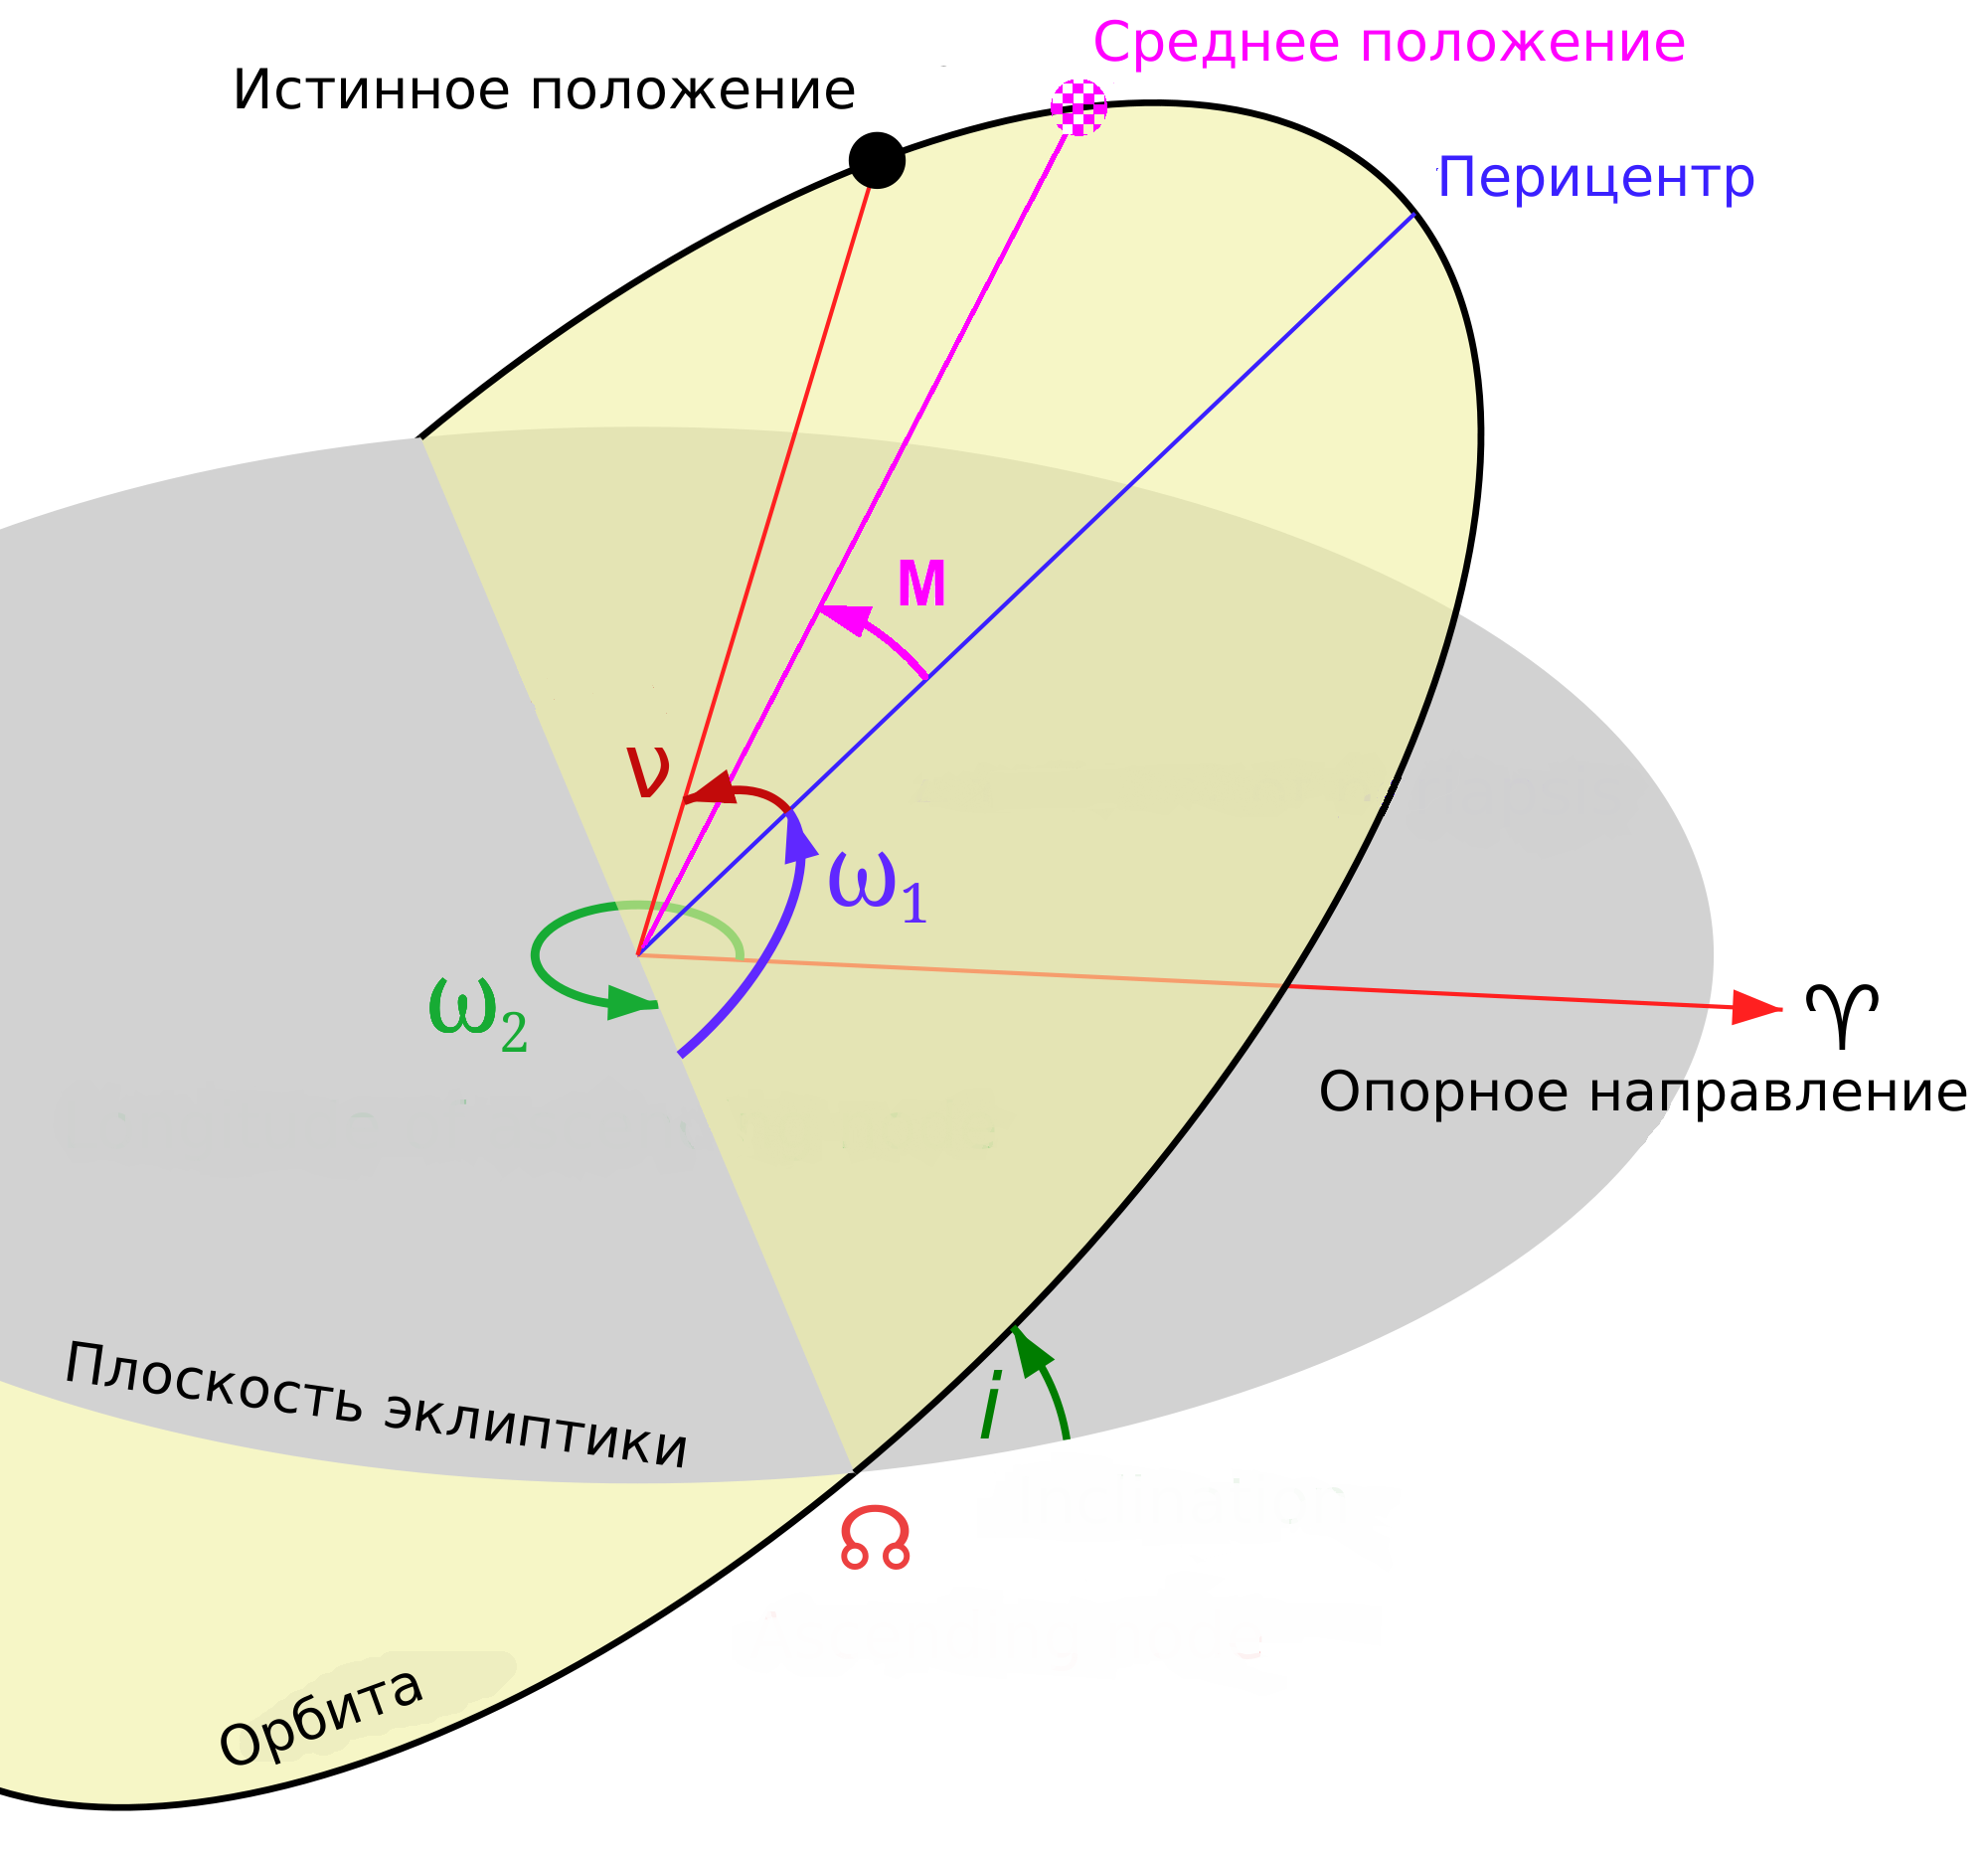
\includegraphics[scale=0.12]{../img/Orbit1-mean.png}
\caption{Средняя долгота $l = \omega_1 + \omega_2 + M$, где $M$ - средняя аномалия}
\end{figure}

Резонанс возникает когда аргументы косинусов близки к стационарным \cite{wis2}:
$$s l + p l_J + j \omega_1 + k \omega_2 + m \omega_{1J} + n \omega_{2J} = \text{const}.$$

Учитывая, что средняя долгота $l$ меняется значительно быстрее остальных углов, получаем резонансное условие (точка обозначает производную по времени):
$$s \dot l + p \dot l_J \approx 0, $$
которое можно переписать в виде:
$$\dot l \approx \frac{-p}{s} \dot l_J \equiv \frac{s+q}{s} \dot l_J.$$

Число $q$ называется порядком резонанса и для исследуемого в данной работе резонанса 3:1 $q=2$, $s=1$.

Учтем, что рассматривается плоская задача, следовательно, $i=0$, $\rho_2=0$, $\omega_2=0$. Подставляя известные коэфициенты ряда и отбрасывая все члены старше второго порядка по $e_J$, получаем \cite{wis2}:
$$H = - \frac{(1-\nu)^2}{2L^2} - \nu R_{sec}(\rho_1, \omega_1) - \nu R_{res}(L,l,\rho_1,\omega_1),$$
где $R_{sec}(\rho_1, \omega_1) = - 2 \rho_1 F - e_J G \sqrt{2 \rho_1} \cos \omega_1$ - секулярная часть возмущающей функции, содержащая медленно меняющиеся со временем члены и в общем случае не периодические, 

$R_{res}(L,l,\rho_1,\omega_1) = 2 \rho_1 C \cos(l-\omega_1-3 l_J)+e_J^2E \cos(l - 3 l_J)$ - резонансная часть возмущающей функции, содержащая медленно изменяющиеся периодические члены.

Масштабным преобразованием можно добиться  \cite{wis2}:
$$a_J=1, \dot l_J= 1 .$$

Производя замену:
$$\Lambda = L - L_{res},$$
$$\lambda = l - 3 l_J,$$
$$x = \sqrt{2 \rho_1} \cos \omega_1,$$
$$y = \sqrt{2 \rho_1} \sin \omega_1,$$
и раскладывая гамильтониан по степеням $\Lambda$, получаем в старшем порядке:
\begin{equation}
\label{Ham_res}
H = \alpha \frac{\Lambda^2}{2} + \nu \left( C(x^2-y^2)+e_J D x + e_J^2 E \right) \cos \lambda + \nu (2Cxy+e_J D y) \sin \lambda + \nu e_J G x + \nu F(x^2+y^2),
\end{equation}
где $L_{res} = \left( \frac{(1-\nu)^2}{3} \right)^\frac13$ - центр резонанса, определяемый условием резонансности 
$$
\dot \lambda = \frac{\partial H}{\partial L}|_{L=L_{res}}=0,$$
a постоянная $\alpha$: 
$$\alpha = -\frac{3(1-\nu)^2}{L_{res}^4} < 0.$$

Следует отметить, что $y$ и $\lambda$ являются координатами, а $x$ и $L$ сопряженными к ним импульсами. При этом фазовое пространство рассматриваемой системы  четырехмерно и, учитывая периодичность правой части уравнений по $\lambda$, можно считать, что:
$$(x,y,\Lambda,\lambda) \in \mathbb{R}^3 \times S^1 .$$

Коэфициенты $F,G,C,D,E,e_J$ являются известными константами, значения которых в случае системы Солнце-Юпитер можно найти, например, в \cite{wis1}.

Систему, описываемую гамильтонианом (\ref{Ham_res}), принято называть плоской эллиптической ограниченной задачей трех тел в случае главного резонанса 3:1.

        \subsection{Практические применения и классичский метод исследования}
        Одним из возможных применений описанной выше задачи является исследование причин возникновения щелей Кирквуда -- определенных областей в поясе астероидов между орбитами Юпитера и Марса, в которых траектории астероидов не могут находиться долгое время. Впервые данные промежутки были обнаружены в 1866 году Д. Кирквудом. Согласно наблюдениям, щели соответствуют целочисленным отношениям периодов орбит астероидов к периоду обращения Юпитера вокруг Солнца. Наиболее отчетливо различимы щели с отношениями: 2:1, 3:1, 5:2, 7:3. 

\begin{figure}[H]
\centering
\includegraphics[scale=0.6]{../img/gaps.png}
%\caption{Щели Кирквуда \cite{graph}}
\caption{Щели Кирквуда}

\end{figure}

\begin{figure}[H]
\centering
\includegraphics[scale=0.25]{../img/gaps2.png}
%\caption{Астероиды в Солнечной системе \cite{plot}}
\caption{Астероиды в Солнечной системе} 

\end{figure}

Большой вклад в исследование данного вопроса внес Д. Висдом, предложивший использовать метод усреднения для объяснения данного эффекта. Рассмотрим канонические уравнения для описанного выше гамильтониана \cite{wis1}:
\begin{equation}
    \begin{cases}
        \frac{d \Lambda}{dt} = \nu \big( U(x,y) \sin \lambda - V(x,y) \cos \lambda \big), \\
        \frac{d \lambda}{dt} = \alpha \Lambda,\\
        \frac{dx}{dt} = -\nu \left(2Fy+\frac{\partial U(x,y)}{\partial y} \cos \lambda + \frac{\partial V(x,y)}{\partial y} \sin \lambda \right), \\
        \frac{dy}{dt} = \nu \left( 2Fx+e_JG +\frac{\partial U(x,y)}{\partial x} \cos \lambda + \frac{\partial V(x,y)}{\partial x} \sin \lambda \right),
    \end{cases}
    \label{sys2}
\end{equation}
где введены обозначения
$$U(x,y) = C(x^2-y^2)+e_J Dx +e_J^2E,$$
$$V(x,y) = 2Cxy+e_JDy.$$

Так как $\frac{dx}{dt}$ и $\frac{dy}{dt}$ пропорциональны $\nu$, то характерное время изменения переменных $x$ и $y$ имеет порядок $\nu^{-1}$, что заметно больше времени малоамплитудных колебаний $\lambda$ (их характерное время порядка $\nu^{-\frac12}$). В силу этого, $x$ и $y$ можно разделить в сумму длинно- и короткопериодных частей: $x=\overline x + \xi$, $y=\overline y + \eta$, причем длиннопериодная часть описывается усредненной системой уравнений:
\begin{equation}
    \begin{cases}
        \frac{d \overline x}{dt} = -\nu \left( 2F \overline y+\frac{\partial U(\overline x,\overline y)}{\partial \overline y} <\cos \lambda> + \frac{\partial V(\overline x,\overline y)}{\partial \overline y} <\sin \lambda> \right), \\
        \frac{d \overline y}{dt} = \nu \left( 2F \overline x+e_JG +\frac{\partial U(\overline x,\overline y)}{\partial \overline x} <\cos \lambda> + \frac{\partial V(\overline x,\overline y)}{\partial \overline x} <\sin \lambda> \right),
    \end{cases}
\end{equation}
где усреднение идет по периоду колебаний $T$:
$$<\cos \lambda>= \frac{1}{T} \int_0^T \cos \lambda dt = 
    \begin{cases} 
        \frac{2E(k_L)}{K(k_L)} - 1, &  -\sqrt{U^2+V^2} < H < \sqrt{U^2+V^2},\\
        \frac{2E(k_C)}{k_C^2 K(k_C)} + 1 - \frac{2}{k_C^2}, & H < -\sqrt{U^2+V^2},
    \end{cases}$$
$$<\sin \lambda>= \frac{1}{T} \int_0^T \sin \lambda dt = 0,$$
$$
k_L = \sqrt{\frac{\nu \sqrt{U^2+V^2} - H}{2 \nu \sqrt{U^2+V^2}}},\quad
k_C = \sqrt{\frac{2 \nu \sqrt{U^2+V^2}}{\nu \sqrt{U^2+V^2} - H}},
$$
$K(k)$ - полный эллиптический интеграл 1 рода,
$E(k)$ - полный эллиптический интеграл 2 рода.

Метод усреднений позволяет понизить число степеней свободы в полной системе до 1 так, что усредненная система становится интегрируемой в силу наличия интеграла движения - усредненного гамильтониана. 

Несмотря на свои преимущества, данный метод применим не для всех областей фазового пространства. В частности он перестает работать в том случае, когда период колебаний $\lambda$ становится сопоставим с периодами $\overline x$ и $\overline y$. Это происходит когда $\frac{d \lambda}{dt} = O(\nu)$ и, соответственно, сопоставимо с $\frac{dx}{dt}$ и $\frac{dx}{dt}$ в силу малости параметра $\nu$. Таким образом, для траектории системы при каждом прохождении в окрестности нулей функции $U(x,y)\sin \lambda - V(x,y) \cos \lambda$ изменяется значение (квази) адиабатического инварианта действия.

    \section{Быстро-медленные системы, медленное многообразие}
        \subsection{Представление плоской эллиптической ограниченной задачи трех тел в окрестности резонанса 3:1 в виде быстро-медленной системы}
        Следует отметить, что уравнения резонансной системы (\ref{Ham_res}) могут быть приведены к виду быстро-медленной системы. Для этого сделаем несимплектическую замену $\Lambda = \sqrt \nu \Lambda_{new}$, $t_{new} = \sqrt \nu t$, после которой канонические уравнения системы примут вид:

\begin{equation*}
    \left\{
    \begin{aligned}
        \frac{d \Lambda_{new}}{dt_{new}} &= U  \sin \lambda - V \cos \lambda, 
        &\quad
        \frac{d \lambda}{dt_{new}} &= \alpha \Lambda_{new}, \\[1.5ex]
        \frac{dx}{dt_{new}} &= -\sqrt \nu \big( 2Fy+\frac{\partial U}{\partial y} \cos \lambda + \frac{\partial V}{\partial y} \sin \lambda \big), 
        &\quad
        \frac{dy}{dt_{new}} &= \sqrt \nu \big( 2Fx+e_JG +\frac{\partial U}{\partial x} \cos \lambda + \frac{\partial V}{\partial x} \sin \lambda \big).
    \end{aligned}
    \right.
\end{equation*}

В дальнейшем для удобства мы будем опускать индекс $new$. Введем новый малый параметр $\varepsilon = \sqrt \nu$. Тогда уравнения принимают итоговый вид (точка обозначает производную по $t$):

\begin{equation}
    \left\{
    \begin{aligned}
        \dot \Lambda &= U \sin \lambda - V \cos \lambda,
        &\quad
        \dot \lambda &= \alpha \Lambda, \\[1.5ex]
        \dot x &= -\varepsilon \big( 2Fy+\frac{\partial U}{\partial y} \cos \lambda + \frac{\partial V}{\partial y} \sin \lambda \big),
        &\quad
        \dot y &= \varepsilon \big( 2Fx+e_JG +\frac{\partial U}{\partial x} \cos \lambda + \frac{\partial V}{\partial x} \sin \lambda \big). \\
    \end{aligned}
    \right.
    \label{fullt}
\end{equation}

Пару переменных $\lambda$ и $\Lambda$ будем называть быстрыми переменными, а пару $x$ и $y$ называть медленными переменными.

        \subsection{Медленное многообразие}
        Медленное многообразие для системы (\ref{fullt}) представляет собой множество:
$$M_0 = \{(x, y, \lambda, \Lambda): \Lambda = 0, u(x,y) \sin \lambda = v(x,y) \cos \lambda \}.$$

Условие $U \sin \lambda = V \cos \lambda$ эквивалентно $\lambda = \arctan(V/U) + \pi k$, $k \in \mathbb{Z}$. Для устранения разрывов при $U = 0$ вводятся две непрерывные функции $\lambda_{\pm}: \mathbb{R}^2 \setminus \{U=V=0\} \to S^1$, отличающиеся на $\pi$:
$$
\lambda_{+}(x,y) \equiv \begin{cases} 
        \arctan \frac{V}{U},        &  U>0, V > 0, \\
        \arctan \frac{V}{U} + \pi,  &  U<0, \\
        \arctan \frac{V}{U} + 2\pi, &  U>0, V<0,
       \end{cases}
\quad
\lambda_{-}(x,y) \equiv \begin{cases} 
        \arctan \frac{V}{U} + \pi,  &  U>0, V > 0, \\
        \arctan \frac{V}{U} + 2\pi, &  U<0, \\
        \arctan \frac{V}{U} + 3\pi, &  U>0, V<0.
       \end{cases}
$$

В особых точках, где $U = V = 0$, решение дает две окружности:
$$y=0,\quad x=x_b^{\pm}\equiv\frac{-e_JD \pm e_J \sqrt{D^2-4EC}}{2C},\quad \Lambda=0,\quad \lambda\in S^1.$$

Локально вблизи этих точек медленное многообразие имеет структуру винтовой поверхности, описываемой уравнением $\tan\lambda = y/(x-x_b^{\pm})$.

\begin{figure}[H]
\centering
\includegraphics[scale=0.55]{../img/MM.png}
\caption{}
\end{figure}

Таким образом, медленное многообразие представляет собой два листа $M_{0,\pm}$, соединенных двумя перемычками $M_{0,b}^{\pm}$:

\begin{align*}
M_0 &= M_{0,+} \cup M_{0,-} \cup M_{0,b}^{+} \cup M_{0,b}^{-}, \\
M_{0,\pm} &= \{ \lambda = \lambda_{\pm}(x,y), \Lambda = 0, (x,y) \in \mathbb{R}^2 \setminus \{U=V=0\} \}, \\
M_{0,b}^{\pm} &= \{ y=0, x=x_b^{\pm}, \Lambda=0, \lambda\in S^1 \}.
\end{align*}

Листы $M_{0,\pm}$ гомеоморфны плоскости с двумя выколотыми точками, а перемычки $M_{0,b}^{\pm}$ - окружностям.

        \subsection{Динамика быстрой системы}
        Устремив в (\ref{fullt}) $\varepsilon$ к нулю, получаем так называемую "быструю"\, систему:

\begin{equation}
    \left\{
    \begin{aligned}
        \dot \Lambda &= U(x,y) \sin \lambda - V(x,y) \cos \lambda,
        &\quad
        \dot \lambda &= \alpha \Lambda, \\[1.5ex]
        \dot x &= 0,
        &\quad
        \dot y &= 0.
    \end{aligned}
    \right.
    \label{fastreal}
\end{equation}

В силу тривиальной динамики переменных $(x, y)$ зависимость функций $U, V$ от медленных переменных будем опускать. Продифференцировав $\lambda$ второй раз по $t$ и подставляя выражение для $\dot \Lambda$, получаем уравнение:
$$\ddot \lambda - \alpha U \sin \lambda + \alpha V \cos \lambda = 0,$$
которое приводится (учитывая $\alpha < 0$) к стандартному уравнению маятника:
$$\ddot \lambda - \alpha \beta \sin \big( \lambda - \lambda_{+}(x,y) \big) = 0, \quad \beta(x,y) \equiv \sqrt{U^2+V^2} > 0.$$

Отметим, что по определению медленное многообразие является множеством неподвижных точек (положений равновесия) "быстрой"\, системы, а именно 
$(\lambda, \Lambda)  = (\lambda_{\pm}(x,y), 0)$. Для определения типа этих положений равновесия разложим правую часть уравнений (\ref{fastreal}) по формуле Тейлора в окрестности положений равновесия:
$$\begin{pmatrix}
  U \sin \lambda - V \cos \lambda \\
  \alpha \Lambda
 \end{pmatrix}
 =
 \begin{pmatrix}
  0 & \alpha \\
  \pm \beta(x,y) & 0
 \end{pmatrix}
 \begin{pmatrix}
  \lambda - \lambda_{\pm}\\
  \Lambda
 \end{pmatrix} + O((\lambda - \lambda_{\pm})^2, \Lambda^2).
$$

Тогда собственные числа линеаризованной системы имеют вид:
\newline
для листа $M_{0,+}$:
$$\zeta = \pm i \sqrt{|\alpha| \beta},$$
\newline
для листа $M_{0,-}$:
$$\zeta = \pm \sqrt{|\alpha| \beta}.$$
В первом случае собственные значения чисто мнимые, а во втором - вещественные. 

Таким образом, лист $M_{0,+}$ состоит из устойчивых положений равновесия быстрой системы,  а лист $M_{0,-}$  - из неустойчивых положений равновесия. Неустойчивое положение равновесия обладает двумерной сепаратрисой, заполненной решениями вида:
\begin{align*}
&\lambda(t, t_0) = \pm 2 \arctan \sinh \big( \alpha \beta (t-t_0) \big) + \lambda_{-}(x,y),\\
&\Lambda(t, t_0) = \frac{\pm 2 \beta}{\cosh \big( \alpha \beta (t-t_0) \big)},
\end{align*}
здесь $t_{0}\in \mathbb{R}$, а выбор знака определяет направление движения по сепаратрисе.

        \subsection{Динамика медленной системы на медленном многообразии}
        Заменив время на медленное $\tau = \varepsilon t$ в уравнениях (\ref{fullt}), получим (штрихом обозначается производная по $\tau$):
\begin{equation}
    \left\{
    \begin{aligned}
        \varepsilon \Lambda' &= U \sin \lambda - V \cos \lambda,
        &\quad
        \varepsilon \lambda' &= \alpha \Lambda,\\
        x' &= - \big( 2Fy+\frac{\partial U}{\partial y} \cos \lambda + \frac{\partial V}{\partial y} \sin \lambda \big),
        &\quad
        y' &= 2Fx+e_JG +\frac{\partial U}{\partial x} \cos \lambda + \frac{\partial V}{\partial x} \sin \lambda.
    \end{aligned}
    \right.
    \label{fulltau}
\end{equation}

Устремив $\varepsilon$ к нулю, получаем "медленную"\, систему:
\begin{equation}
    \left\{
    \begin{aligned}
        0 &= U \sin \lambda - V \cos \lambda,
        &\quad
        0 &= \alpha \Lambda, \\
        x' &= -\big( 2Fy+\frac{\partial U}{\partial y} \cos \lambda + \frac{\partial V}{\partial y} \sin \lambda \big),
        &\quad
        y' &= 2Fx+e_JG +\frac{\partial U}{\partial x} \cos \lambda + \frac{\partial V}{\partial x} \sin \lambda.
    \end{aligned}
    \right.
    \label{slowreal}
\end{equation}

Подставляя в (\ref{slowreal}) введенную ранее параметризацию листов медленного многообразия, получаем:
\begin{equation}
    \left\{
    \begin{aligned}
        x' &= - \big( 2Fy \pm \frac{\partial \beta}{\partial y} \big),
        &\quad
        y' &= 2Fx+e_JG \pm \frac{\partial \beta}{\partial x}.
    \end{aligned}
    \right.
    \label{slow_sys}
\end{equation}
Знаки "$+$" и "$-$" соответсвуют $M_{0,+}$ и $M_{0,-}$ соответственно.

Данная система является гамильтоновой с гамильтонианом:
$$H_S = F(x^2+y^2) + e_JGx \pm \beta(x,y),$$
и имеет одну степень свободы, что приводит к ее интегрируемости.

На каждом из листов медленного многообразия такая система единственное положение равновесия:
$$
y_0^{\pm} = 0,\quad
x_0^{\pm} = \frac{e_J (\pm D - G)}{2(F \mp C)}.
$$

Линеаризуя правую часть уравнений в окрестности этой точки, получаем что собственные значения матрицы линеаризации имеют вид:
$$\zeta = \pm \sqrt{- \left( 2F \pm 2C \pm \frac{2Cx_0^{\pm}+e_JD}{|U(x_0^{\pm},0)|} \right)\big( 2F \mp 2C \big)} \in \mathbb{R},$$
причем, учитывая значения констант, они являются чисто вещественными, что позволяет сказать о неустойчивости данного положения равновесия на обоих листах.

Как и в случае маятника, эти неустойчивые положения равновесия обладают двумерными сепаратрисами, заполненными сепаратрисными решениями, асимптотически приближающимися к положениям равновесия при $\tau\to \pm\infty$. Для их нахождения рассмотрим линию критического уровня гамильтониана $H_S(x,y) = H_S(x_0^{\pm},y_0^{\pm})$, соответствующего неподвижной точке:
$$H_S(x_0^{\pm},y_0^{\pm}) = F(x^2+y^2)+e_JGx \pm \beta(x,y).$$

\begin{figure}[H]
\centering
\includegraphics[scale=0.4]{../img/Hlines.png}
\caption{Линии уровня гамильтониана $H_S$ на $M_{0,+}$. На $M_{0,-}$ линии уровня имеют аналогичный вид}
\label{levels_slow}
\end{figure}

Сделав замену $x = x_0^{\pm} + h$ и упростив выражение, получаем:
\begin{multline}
(F^2-C^2)(h^2+y^2)^2+2(h^2+y^2) \big(U(x_0^{\pm}, y_0)+h(2Cx_0^{\pm}+e_JD) \big) (\pm F - C)+\\ 
+ y^2 \big(4U(x_0^{\pm},y_0^{\pm})C-(2Cx_0^{\pm}+e_JD)^2 \big) = 0.
\label{eight}
\end{multline}
Сделаем инверсию относительно единичной окружности: $X=\frac{h}{h^2+y^2}$, $Y=\frac{y}{h^2+y^2}$. Тогда уравнение (\ref{eight}) принимает вид:
$$(F^2-C^2)+AX^2+2BX+(A+\delta)Y^2=0,$$
где
$$A = 2 U(x_0^{\pm}, y_0^{\pm})(\pm F - C),$$
$$B = (2Cx_0^{\pm}+e_J D)(\pm F - C),$$
$$\delta = -(2Cx_0^{\pm}+e_J D)^2.$$
Если ввести новые переменные:
$$\xi  = \left( X+\frac{B}{A} \right) \sqrt{\frac{A}{F^2-C^2-\frac{B^2}{A}}} \equiv \omega \left( X+\frac{B}{A} \right),$$
$$\eta = Y \sqrt{\frac{-(A+\delta)}{F^2-C^2-\frac{B^2}{A}}} \equiv \sigma Y,$$
то уравнение критического уровня может быть переписано следующим образом:
\begin{equation}
\label{hyper}
\xi^2-\eta^2=1.
\end{equation}
Таким образом, в переменных $(\xi, \eta)$ линия уровня гамильтониана $H_S(x,y) = H_S(x_0^{\pm},y_0^{\pm})$ есть гипербола. В первоначальных переменных  $(x, y)$, т.е. до инверсии относительно единичной окружности, данная кривая имеет форму "восьмерки"\, (см. рис. \ref{levels_slow}).

Введем следующую параметризацию полученной кривой с помощью переменной $f$:
$$\xi = \ch f,$$
$$\eta = \sh f,$$
$$\xi^2-\eta^2 = \ch^2f - \sh^2f = 1.$$
Теперь для нахождения сепаратрисного решения необходимо определить зависимость $f$ от времени $\tau$. Для этого рассмотрим:
\begin{equation}
\label{der_x_1}
x' = \frac{\partial x}{\partial X}X'+\frac{\partial x}{\partial Y}Y' = \frac{Y^2-X^2}{(X^2+Y^2)^2}X' + \frac{-2XY}{(X^2+Y^2)^2}Y' = f' \sh f \frac{Q(\ch f)}{P^2(\ch f)},
\end{equation}
где
$$P(\ch f) \equiv X^2+Y^2 = \ch^2 f \left( \frac{1}{\omega^2} + \frac{1}{\sigma^2} \right) + \frac{-2B }{\omega A}\ch f + \left( \frac{B^2}{A^2}-\frac{1}{\sigma^2} \right),$$

$$Q(\ch f) \equiv  -\frac{\ch^2 f}{\omega} \left( \frac{1}{\omega^2}+\frac{1}{\sigma^2} \right) + \frac{2B}{A} \ch f \left( \frac{1}{\sigma^2}+\frac{1}{\omega^2} \right) - \frac{1}{\omega} \left( \frac{1}{\sigma^2} + \frac{B^2}{A^2} \right).$$

С другой стороны, подставляя (\ref{eight}) в первое уравнение системы (\ref{slow_sys}), получаем:

$$x' = -\left( 2Fy \pm \frac{\partial \beta}{\partial y} \right) = -2Fy \mp \frac{1}{\beta} \left( U \frac{\partial U}{\partial y} + V \frac{\partial V}{\partial y} \right) = $$

$$ = \frac{y \Big(2(C^2-F^2)(x^2+y^2) + 2x(2Cx_0+e_J D)(C \mp F) + (2Cx_0+e_J D)^2 + 2U(x_0, y_0)(-C \mp F)  \Big)}{F(x^2+y^2) \pm U(x_0, y_0) \pm x(2Cx_0+e_J D)}.$$

Тогда в терминах переменной $f$ получаем
\begin{equation}
\label{der_x_2}
x' = \frac{\sh f}{\sigma P(\ch f)} \frac{R(\ch f)}{S(\ch f)},
\end{equation}
где
$$R(\ch f) \equiv P(\ch f) \left( 2 U(x_0,y_0)(-C \mp F)+(2Cx_0+e_J D)^2 \right) +$$ 
$$ + 2 \left( \frac{\ch f}{\omega} - \frac{B}{A} \right)(2Cx_0 + e_J D)(C \mp F) + 2(C^2-F^2),$$
$$S(\ch f) \equiv \pm U(x_0,y_0) P(\ch f) \pm \left( \frac{\ch f}{\omega} - \frac{B}{A}\right) (2Cx_0+e_J D) + F.$$
Сравнивая выражения (\ref{der_x_1}) и (\ref{der_x_2}), получаем дифференциальное уравнение на $f$:
\begin{equation}
\label{der_f}
f' = \frac{1}{\sigma} \frac{R(\ch f) P(\ch f)}{S(\ch f)Q(\ch f)}.
\end{equation}
Заметим, что $P, Q, R, S$ являются полиномами второго порядка переменной $\ch f$.
Интегрируя уравнение (\ref{der_f}), имеем:
\begin{equation*}
\tau -\tau_0 = \sigma \int_{f_0}^f \frac{S(\ch f) Q(\ch f)}{R(\ch f)P(\ch f)} df = 
\end{equation*}
\begin{equation} = (f-f_0)\frac{\mp 2U(x_0^{\pm}, y_0^{\pm}) \frac{\sigma}{\omega}}{2U(x_0^{\pm},y_0^{\pm})(-C \mp F)+(2Cx_0^{\pm} + e_J D)^2} + \sigma \int_{f_0}^f \frac{L(\ch f)}{R(\ch f) P(\ch f)} df,
\label{f_tau}
\end{equation}
где $L$ некоторый полином 3 степени.

\begin{utv}
На обоих листах $M_{0,k}, k=+,-$ медленная система (\ref{slow_sys}) имеет неустойчивое положение равновесия $(x,y) = (x_0^{\pm},y_0^{\pm})$. Это положение равновесия порождает двумерную сепаратрису, заполненную решениями вида:
$$x(\tau,\tau_{0}) = x_0 + \frac{\frac{\ch \big( f(\tau-\tau_{0}) \big)}{\omega} - \frac{B}{A}}{P \Big(\ch \big( f (\tau-\tau_{0}) \big) \Big)},$$
$$y(\tau, \tau_{0}) = \frac{\sh \big( f(\tau-\tau_{0}) \big)}{\sigma P\Big(\ch \big( f (\tau-\tau_{0}) \big) \Big)},$$
где $\tau_{0}\in \mathbb{R}$, а функция $f(\tau)$ задается выражением (\ref{f_tau}).
\end{utv}

        \subsection{Неподвижные точки полной системы}
        Заметим, что точка $(\hat x^{-}_0, 0, \lambda_{-}(\hat x^{-}_0, 0), 0)$ является положением равновесия не только быстрой системы (т.к. принадлежит медленному многообразию), но также является неподвижной точкой для полной системы. Линеаризация в окрестности этой точки показывает, что данное положение равновесия имеет тип \textit{седло-седло} (матрица Якоби имеет четыре вещественных собственных значения, два из которых положительны, а два отрицательны).


Неподвижная точка медленной системы $(\hat x^{+}_0, 0, \lambda_{+}(\hat x^{+}_0, 0), 0) \in M_{0,+}$, аналогично случаю неустойчивого листа, также является положением равновесия полной системы (\ref{fullt}). Линеаризация показывает, что эта точка имеет тип \textit{седло-центр} с собственными значениями $(\pm i \omega, \pm \xi)$.
    \begin{align*}
    \omega &= \frac{\sqrt{\sqrt p - q}}{\sqrt 2} = \sqrt{|\alpha U(\hat x_0^+,0)|} + \mathcal{O}(\varepsilon^2), \\
    \xi &=    \frac{\sqrt{\sqrt p + q}}{\sqrt 2} = \mathcal{O}(\varepsilon),
    \label{eigenval}
    \end{align*}
    $$p = (4 \varepsilon^2(C-F)(C+F) + \alpha U(\hat x_0^+,0))^2 + 8 \alpha \varepsilon^2 (F-C) V_y(\hat x_0^+,0) > ,0$$
    $$q = 4 \varepsilon^2 (C-F)(C+F) - \alpha U(\hat x_0^+,0) < 0.$$    


    Положение равновесия типа \textit{седло-центр} имеет одномерные устойчивое и неустойчивое многообразия и двумерное центральное многообразие. В общем случае, если устойчивое и неустойчивое многообразия пересекаются, то они совпадают и могут быть параметризованы гомоклинической траекторией. Поскольку эти одномерные устойчивое и неустойчивое многообразия лежат в трехмерном уровне энергии и гладко зависят от $\varepsilon$, следует ожидать, что система будет иметь изолированные значения малого параметра, при которых  устойчивое и неустойчивое многообразия пересекаются.

       
        
    \section{Динамика в окрестности неустойчивого листа}
        \subsection{Инвариантные многообразия}
        \subsubsection{Основные понятие и теоремы}

Одним из методов анализа поведения траекторий системы вблизи медленного многообразия является  геометрическая теория возмущений Феничеля. 
В этом параграфе мы сформулируем некоторые определения и теоремы теории гиперболических множеств и теории Феничеля.

\begin{dfn}
Говорят, что компактное, $C^r$-гладкое, связное многообразие с краем $M \subset R^n$ инвариантно назад (вперёд) относительно потока $\theta_t (x)$, порождённого системой $\frac{dx}{dt} = F(x)$ ($x \in \mathbb{R}^n$, $F(x)$ - $C^r$-гладкое векторное поле), если для всякого $p \in M$ поток $\theta_t (p) \in M$ при $t \leq 0$ 
($t \geq 0$) и для всякого $p \in \partial M$ поле $-F(p)$  направлено внутрь $M$. 

Говорят, что многообразие $M$ инвариантно относительно потока $\theta_t (x)$, если оно одновременно является локально инвариантным вперёд и назад.
\end{dfn}

\begin{dfn}
Компактное, $C^r$-гладкое, связное многообразие с краем $M \subset \mathbb{R}^n$ локально инвариантно относительно потока $\theta_t (x)$, если для всякого $p \in M \setminus \partial M$ найдется интервал $(t_1,t_2)$, $t_1<0$, $t_2>0$ такой, что для любого $t \in (t_1,t_2)$ верно $\theta_t(p) \in M$.
\end{dfn}

\begin{dfn}
Инвариантное множество $M$ называется гиперболическим, если для всякого 
$x_0 \in M$ существуют $\lambda_{1,2} > 0$ такие, что:
$$T_{x_0}\mathbb{R}^{n} = T_{x_0} M \oplus E_{x_0}^u \oplus E_{x_0}^s ,$$
$$\forall v \in E_{x_0}^s, (T_{x_0} \theta_t)v \in E_{\theta_t(x_0)}^s \Rightarrow ||(T_{x_0} \theta_t)v|| \leq e^{-\lambda_1 t} ||v||,\,\, t \geq 0 ,$$
$$\forall v \in E_{x_0}^u, (T_{x_0} \theta_t)v \in E_{\theta_t(x_0)}^u \Rightarrow ||(T_{x_0} \theta_t)v|| \leq e^{\lambda_2 t} ||v||,\,\, t \leq 0 .$$
\end{dfn}

\begin{thm}
\textbf{(Адамар-Перрон):}

Если $M$ - инвариантное гиперболическое множество, то существуют единственные инвариантные устойчивое и неустойчивое многообразия, определеляемые следующим образом:
$$W^s(M) = \{ x: \text{dist} \big(\theta_t(x), M \big) \rightarrow 0, t \rightarrow +\infty \},$$
$$W^u(M) = \{ x: \text{dist} \big(\theta_t(x), M \big) \rightarrow 0, t \rightarrow -\infty \}.$$
\end{thm}

Сформулируем теперь понятие гиперболичности для локально инвариантных множеств:

\begin{dfn}
Локально инвариантное множество $M$ называется гиперболическим, если для всякого $x_0 \in M$ существуют $\lambda_{1,2} > 0$ такие, что:
$$T_{x_0}\mathbb{R}^{n} = T_{x_0} M \oplus E_{x_0}^u \oplus E_{x_0}^s ,$$
$$\forall v \in E_{x_0}^s, (T_{x_0} \theta_t)v \in E_{\theta_t(x_0)}^s \Rightarrow ||(T_{x_0} \theta_t)v|| \leq e^{-\lambda_1 t} ||v||, 0\le t < t_{2} ,$$
$$\forall v \in E_{x_0}^u, (T_{x_0} \theta_t)v \in E_{\theta_t(x_0)}^u \Rightarrow ||(T_{x_0} \theta_t)v|| \leq e^{\lambda_2 t} ||v||, t_{1} < t \le 0 .$$
\end{dfn}

В этом случае справедлив аналог теоремы Адамара-Перрона \cite{berger}

\begin{thm}

Если $M$ - локально инвариантное гиперболическое множество, то существуют локально инвариантные устойчивое и неустойчивое многообразия, определеляемые следующим образом:
$$W^s(M) = \{ x: \text{dist}(\theta_t(x), M) \le \text{dist}(x, M), 0\le t < t_{2} \},$$
$$W^u(M) = \{ x: \text{dist}(\theta_t(x), M) \le \text{dist}(x, M), t_{1} <  t \le 0 \}.$$
\end{thm}

Можно заметить, что инвариантные (локально инвариантные) устойчивое и неустойчивое многообразия расслаиваются на траектории (конечные сегменты траекторий). Дадим следующее

\begin{dfn}
Пусть $M_1$, $M_2$ - два (локально) инвариантных гиперболических множества, $W^{s,u}(M_{1,2})$ - соответствующие им устойчивое и неустойчивое многообразия. Тогда точка $x_0 \in W^u(M_1) \cap W^s(M_2)$ называется гомоклинической, если $M_1 = M_2$, и гетероклинической если $M_1 \neq M_2$. Соответствующие траектории $\theta_t(x_0) \in W^u(M_1) \cap W^s(M_2)$ называются (локально) двояко-асимптотическими.
\end{dfn}

\begin{dfn}
Гомоклиническая (гетероклиническая) точка $x_0$ называется трансверсальной, если:
$$T_{x_0}\mathbb{R}^{n} = T_{x_0}W^s(M_1) \oplus T_{x_0}W^u(M_2).$$
\end{dfn}

Следующая теорема является важным результатом сингулярной теории возмущений:

\begin{thm}
\textbf{(Феничель, \cite{fenichel}):}

Пусть $M_0$ компактное локально инвариантное гиперболическое множество относительно потока $\theta_{t}^{(0)}$, определяемого векторным полем $F_{0}$. Рассмотрим для $\delta>0$ локальные устойчивое и неустойчивое многообразия $W_{loc}^{(s,u)}(M_0) = W_{loc}^{(s,u)}(M_0)\cap U_{\delta}(M_0)$.
Тогда существует достаточно малое $\varepsilon_{0} > 0$ такое, что для любого векторного поля $F_{\varepsilon}$, удовлетворяющего $\vert F_{\varepsilon} - F_{0}\vert < \varepsilon < \varepsilon_{0}$ существует локально инвариантное множество $M_{\varepsilon}$, лежащее в $\varepsilon$ окрестности $M_0$, локально инвариантные устойчивое и неустойчивое многообразия которого $O(\varepsilon)$ близки к 
$W_{loc}^{s,u}(M_0)$.
\end{thm}

Следствием этой теоремы является следующая
\begin{thm}
\textbf{(Феничель, \cite{jones}):}

Пусть $M_0$ компактное подмногообразие (возможно с границей) медленного многообразия системы (\ref{fullt}), гиперболическое относительно (\ref{fast}).

Тогда для любого достаточно малого $\varepsilon > 0$ существует локально инвариантное многообразие $M_{\varepsilon}$ системы (\ref{fullt}) , лежащее в 
$\varepsilon$ окрестности $M_0$.
\end{thm}

Заметим, что данные теоремы гарантируют существование лишь локально инвариантных множеств, вопрос существования глобально инвариантных множеств является более сложной задачей.

Для невозмущенной системы двояко-асимптотические траектории лежат в пересечении устойчивого и неустойчивого многообразий $W^s(M_0) \cap W^u(M_0)$. То же верно и для возмущенной системы, однако, если множество $M_{0}$ имеет непустую границу, то теория Феничеля гарантирует существование лишь локально инвариантных устойчивого и неустойчивого многообразий. Таким образом, их пересечение $W^s(M_\varepsilon) \cap W^u(M_\varepsilon)$ - это множество траекторий, которые ведут себя как гомоклинические только на некотором ограниченном интервале времени.

В дальнейшем будет показано, что существует множество, остающееся глобально инвариантным при возмущении.




        \subsection{Метод Мельникова}
        %\subsection{Трансверсальные пересечения устойчивого и неустойчивого многообразий}

Трансверсальные гомоклинические и гетероклиническое траектории являются важными объектами в теории гладких динамических систем. Наличие таких траекторий приводит к сложной хаотической динамике и, как следствие, к неинтегрируемости исследуемой системы. 

Для нахождения пересечений устойчивого и неустойчивого многообразий применим метод Мельникова. Рассмотрим систему уравнений вида:
\begin{equation}
    \begin{cases}
        \frac{dX}{dt} = J D_X H_1(X,I) + \varepsilon g^X(X,I), \\
        \frac{dI}{dt} = \varepsilon g^I(X,I),
    \end{cases}
    \label{wiggs}
\end{equation}
$$X \in \mathbb{R}^2, I \in \mathbb{R}^m,$$


где $D_X, D_I$ - градиенты по соответствующим переменным, $J$ - симплектическая единица:
$$
 J = \begin{pmatrix}
  0  & 1 \\
  -1 & 0
 \end{pmatrix}.
$$

\begin{thm}
\textbf{(Функция Мельникова \cite{wiggins}):}

Пусть $V \subset M_0$ - инвариантное гиперболическое подмножество медленного многообразия $M_0$ системы (\ref{wiggs}), за $V_\varepsilon$ обозначено локально инвариантное множество лежашее в $\varepsilon$-окрестности $V$, существовние которго гарантирует теорема Феничеля.

$$\Gamma = W^s(V) \cap W^u(V) \setminus V$$

%Пусть $X = \gamma(I)$ - параметризация $V$.

Пусть $X_0^I(t-t_0,I)$ - сепаратриса быстрой системы, соответствующей (\ref{wiggs}).

Тогда расстояние между $W^s(V_\varepsilon)$ и $W^u(V_\varepsilon)$ вблизи любой точки $p \in \Gamma$ задается выражением:

$$d^I(p, t_0, \varepsilon) = \varepsilon\frac{M^I(p,t_0)}{||D_X H(X_0^I, I)||} + O(\varepsilon^2),$$
где $M^I$ - функция Мельникова, равная:

$$M^I(p,t_0) = \int_{-\infty}^{\infty} \Big( <D_X H_1, g^X> + <D_X H_1, (D_I J D_X)\int_{t_0}^t g^I dt > \Big) \big(X_0^I(t-t_0,I),I \big)dt = $$
$$= \int_{- \infty}^{\infty} \Big( <D_X H_1, g^X> + <D_I H_1, g^I> \Big)\big(X_0^I(t-t_0,I), I \big)dt - $$
$$ -<D_I H_1 \big(v(I), I \big), \int_{- \infty}^{\infty} g^I \big(X_0^I(t-t_0,I), I \big)dt>,$$
здесь $X = v(I)$ - параметризация $V$, $<,>$ - стандартное скалярное произведение в $\mathbb{R}^2$.
\end{thm}
\textbf{Доказательство \cite{wiggins}:}
%%%%%%%%%%%%%%%%%%%%%%%%%%%%%%%%%%%%%%%%%%%%%%%%%%%%%%%%%%%
Зафиксируем точку $p \in \Gamma = W^s(V) \cap W^u(V) \setminus V$ и рассмотрим $\Pi_p$ гиперплоскость натянутую на вектор $D_X H_1(p)$.

Тогда в силу теоремы Феничеля (Теорема 3) существуют точки $p_\varepsilon^u \equiv (X_\varepsilon^u, I_\varepsilon^u) \in W^{u}(V_\varepsilon) \cap \Gamma \cap \Pi_p$ и $p_\varepsilon^s \equiv (X_\varepsilon^s, I_\varepsilon^s) \in W^{s}(V_\varepsilon) \cap \Gamma \cap \Pi_p$, причем $I_\varepsilon^s = I_\varepsilon^u$.  

Введем расстояние между $W^s(V_\varepsilon)$ и $W^u(V_\varepsilon)$ как:

$$d(p,t_0, \varepsilon) = ||p_\varepsilon^u - p_\varepsilon^s|| = ||X_\varepsilon^u - X_\varepsilon^s|| = \frac{<D_X H_1 \big(X_0^I(t-t_0,I),I \big),X_\varepsilon^u - X_\varepsilon^s>}{||D_X H_1 \big(X_0^I(t-t_0,I), I \big)||}.$$

Раскладывая его в ряд по $\varepsilon$ в окрестности нуля и учитывая, что $d(p,0) = 0$ в силу того, что $p \in W^s(V) \cap W^u(V)$, получаем:

$$d(p,t_0, \varepsilon) = \varepsilon \frac{<D_X H_1 \big(X_0^I(t-t_0,I),I \big), \frac{\partial X_\varepsilon^u}{\partial \varepsilon}\big|_{\varepsilon = 0} - \frac{\partial X_\varepsilon^s}{\partial \varepsilon}\big|_{\varepsilon = 0}>}{||D_X H_1 \big( X_0^I(t-t_0,I), I \big)||} + O(\varepsilon^2).$$

Числитель дроби называется функцией Мельникова:
$$M^I(p,t_0) = <D_X H_1 \big(X_0^I(t-t_0,I),I \big), \frac{\partial X_\varepsilon^u}{\partial \varepsilon} \Big|_{\varepsilon = 0} - \frac{\partial X_\varepsilon^s}{\partial \varepsilon}\Big|_{\varepsilon = 0}>.$$

Рассмотрим 
$$M(t,t_0) = <D_X H_1 \big(X_0^I(t-t_0,I),I \big), \frac{\partial X_\varepsilon^u(t)}{\partial \varepsilon}\Big|_{\varepsilon = 0} - \frac{\partial X_\varepsilon^s(t)}{\partial \varepsilon}\Big|_{\varepsilon = 0}> = \Delta^u(t) - \Delta^s(t),$$
$$\Delta^{u,s}(t) = <D_X H_1 \big(X_0^I(t-t_0,I),I \big), \frac{\partial x_\varepsilon^{u,s}(t)}{\partial \varepsilon}\Big|_{\varepsilon = 0}>.$$

Производные по $\varepsilon$ в скалярном произведении описываются вариационными уравнениями:

$$\frac{d}{dt} \frac{\partial X_\varepsilon^{u,s}(t)}{\partial \varepsilon}\Big|_{\varepsilon = 0} = J D_X^2 H_1 \frac{\partial X_\varepsilon^{u,s}(t)}{\partial \varepsilon}\Big|_{\varepsilon = 0} + D_I J D_X H_1 \frac{\partial I_\varepsilon^{u,s}(t)}{\partial \varepsilon}\Big|_{\varepsilon = 0} + g^X \big(X_0^I(t-t_0,I), I \big),$$
$$\frac{d}{dt} \frac{\partial I_\varepsilon^{u,s}(t)}{\partial \varepsilon}\Big|_{\varepsilon = 0} = g^I \big(X_0^I(t-t_0,I), I \big).$$

Тогда обозначив:
$$x_1^{u,s}(t) = \frac{\partial X_\varepsilon^{u,s}(t)}{\partial \varepsilon}\Big|_{\varepsilon = 0},$$
$$I_1^{u,s}(t) = \frac{\partial I_\varepsilon^{u,s}(t)}{\partial \varepsilon}\Big|_{\varepsilon = 0},$$
получаем:
$$\frac{d}{dt} \Delta^{u,s}(t) = <\frac{d}{dt} \Big(D_X H_1 \big(X_0^I(t-t_0,I),I\big) \Big), x_1^{u,s}> + <D_X H_1 \big(X_0^I(t-t_0,I),I \big), \frac{d}{dt} x_1^{u,s}> = $$
$$=<D_X H_1, (J D_X^2 H_1) x_1^{u,s}> + <D_X H_1, (D_I J D_X H_1) I_1^{u,s}> + $$
$$ + <D_X H_1, g^X> + <(D_X^2 H_1)(JD_X H_1),x_1^{u,s}>.$$

Учитывая равенство
$$<D_X H_1, (J D_X^2 H_1) x_1^{u,s}> + <(D_X^2 H_1)(JD_X H_1),x_1^{u,s}> = 0,$$
получаем:
$$\frac{d}{dt} \Delta^{u,s}(t) =  <D_X H_1, (D_I J D_X H_1) I_1^{u,s}> + <D_X H_1, g^X>.$$

Из уравнения в вариациях следует:
$$I_1^s(t) = I_1^u(t) = \int_{t_0}^t g^I \big(X_0^I(t-t_0,I), I \big) dt.$$

Проинтегриуем полученные уравнения по $t$:

$$\Delta^u(0) - \Delta^u(-T^u) = \int_{-T^u}^0 \Big( <D_X H_1, g^X> + <D_X H_1, (D_I J D_X)\int_{t_0}^t g^I dt > \Big) \big(X_0^I(t-t_0,I),I \big)dt,$$

$$\Delta^s(T^s) - \Delta^s(0) = \int_{0}^{T^s} \Big( <D_X H_1, g^X> + <D_X H_1, (D_I J D_X)\int_{t_0}^t g^I dt > \Big) \big(X_0^I(t-t_0,I),I \big)dt.$$

В силу локальной инвариантности многообразий $W^{s,u}(V)$ невозможно устремить $T^{s,u}$ к бесконечности, однако, их можно сделать сколь угодно большими. А именно, для любого $\delta>0$ существует $\varepsilon_0$ такое, что для любого 
положительного $\varepsilon < \varepsilon_0$ имеет место оценка $T^{s,u}>\frac{1}{\delta}$.

Заметим, что по построению:
$$M^I(p,t_0) = M^I(t=0,t_0),$$
тогда:
$$M^I(p,t_0) = M^I(t=0,t_0) \approx $$
$$ \approx \int_{-T^u}^{T^s} \Big( <D_X H_1, g^X> + <D_X H_1, (D_I J D_X)\int_{t_0}^t g^I dt > \Big) \big(X_0^I(t-t_0,I),I \big)dt + \Delta^u(-T^u) - \Delta^s(T^s).$$

%\qed
%%%%%%%%%%%%%%%%%%%%%%%%%%%%%%%%%%%%%%%%%%%%%%%%%%%%%%%%%%%

\begin{thm}
\textbf{(Нули функции Мельникова, \cite{wiggins}):}

Если при некоторых значениях аргумента функции Мельникова верно: 
$$M^I = 0,$$
$$\nabla M^I \neq 0.$$
Тогда при достаточно малом $\varepsilon > 0$ $W^s(V_\varepsilon)$ и $W^u(V_\varepsilon)$ пересекаются трансверсально.

В случаях когда и сама функция, и ее градиент обращаются в ноль нужно рассматривать члены при старших степенях $\varepsilon$ в разложении $d^I$ для определения трансверсальности пересечения.

\end{thm}

        \subsection{Применение теории Мельникова к плоской эллиптической ограниченной задаче трех тел}
        В силу Утверждений 1,2 приходим к

\begin{utv}
Для системы (\ref{fullt}) имеют место:

1.  множества 
$$M_0, M_{0,+}, M_{0,-}, M_{0,b}^{\pm}$$
являются инвариантными.

2. Множество $M_{0,-}$ является также гиперболическим.

3. Пусть $\Big( x(t), y(t), 0, \lambda_{-} \big( x(t),y(t) \big), \Lambda = 0 \Big)$ - некоторая траектория медленной системы (\ref{slowreal}) на $M_{0,-}$, тогда окрестность этой траектории на плоскости $xy$ является инвариантным гиперболическим множеством.

\end{utv}

Найдем явный вид функции Мельникова для исследуемой системы. Для этого приведем уравнения (\ref{fullt}) к виду (\ref{wiggs}):
$$
 X = \begin{pmatrix}
  \Lambda\\
  z
 \end{pmatrix},
 I = \begin{pmatrix}
  x\\
  y
 \end{pmatrix}.$$

Переменная $z$ вводится как:
$$z = \lambda - \lambda_{-}(x,y).$$ 
При этом многообразие $M_{0,-}$ переходит в $\tilde M_{0,-}$:
$$\tilde M_{0,-} = \left\{ (\Lambda, z, x, y): \Lambda = 0,\,\, z=0 \right\},$$
а сепаратриса записывается в виде:
$$z_{sep}(t,t_0) = \pm 2 \arctan{\sh \big( \alpha \beta (t-t_0) \big)}, \Lambda_{sep}(t,t_0) = 2\beta/ \ch \big(\alpha \beta (t-t_0) \big).$$

Тогда в терминах новых переменных имеем:
$$
 D_X = \begin{pmatrix}
  \frac{\partial}{\partial \Lambda}\\
  \frac{\partial}{\partial z}
 \end{pmatrix},
 D_I = \begin{pmatrix}
  \frac{\partial}{\partial x}\\
  \frac{\partial}{\partial y}
 \end{pmatrix},
 $$

$$H_1 = \alpha \frac{\Lambda^2}{2}+\beta(x,y)(1-\cos z),\quad \beta(x,y) = \sqrt{u(x,y)^2+v(x,y)^2},$$

$$g^I = \begin{pmatrix}
  -2Fy+\frac{\partial \beta}{\partial y} \cos z + \beta(x,y) \frac{\partial}{\partial y} \arctan(\frac{v}{u}) \sin z\\
  2Fx +e_JG -\frac{\partial \beta}{\partial x} \cos z - \beta(x,y) \frac{\partial}{\partial x} \arctan(\frac{v}{u}) \sin z
 \end{pmatrix},$$

$$g^X = \frac{-1}{\varepsilon} \begin{pmatrix}
  0 \\
  \frac d{dt} \arctan(\frac vu)
 \end{pmatrix}
 = 
 \frac{-(u \dot v - v \dot u)}{\varepsilon \beta^2} \begin{pmatrix}
  0 \\
  1
 \end{pmatrix}
 =
 \frac{-\Big(\dot x \big(u \frac{\partial v}{\partial x} - v \frac{\partial u}{\partial x} \big) + \dot y \big(u \frac{\partial v}{\partial y} - v \frac{\partial u}{\partial y}\big) \Big)}{\varepsilon \beta^2} \begin{pmatrix}
  0 \\
  1
 \end{pmatrix} = 
 $$
 
$$
 =
 \frac{\big(2Fy+\frac{\partial u}{\partial y} \cos \lambda + \frac{\partial v}{\partial y} \sin \lambda \big) \big(u \frac{\partial v}{\partial x} - v \frac{\partial u}{\partial x}\big) - \big(2Fx+e_JG +\frac{\partial u}{\partial x} \cos \lambda + \frac{\partial v}{\partial x} \sin \lambda \big) \big(u \frac{\partial v}{\partial y} - v \frac{\partial u}{\partial y} \big)}{\beta^2} \begin{pmatrix}
  0 \\
  1
 \end{pmatrix}.
 $$

\subsection{Расщепление сепаратрис}

Построим функцию Мельникова для множества $V=\tilde M_{0,-}$ из Теоремы 5.
Для этого сначала отдельно посчитаем подинтегральное выражение:
$$<D_IH_1, g^I> = (1 - \cos z) \Bigg( -2Fy \frac{\partial \beta}{\partial x}+(2Fx+e_J G)\frac{\partial \beta}{\partial y} + \frac{\sin z}{\beta} \bigg( 
\frac{\partial \beta}{\partial y}\Big(v \frac{\partial u}{\partial y}-u \frac{\partial v}{\partial y}\Big)-\frac{\partial \beta}{\partial x}\Big(v \frac{\partial u}{\partial x}-u \frac{\partial v}{\partial x} \Big)   \bigg)    \Bigg),$$

$$<D_XH_1,g^X> = \frac{- \beta  \sin z}{\varepsilon} \frac{d}{dt}{\Big( \arctan \frac{v}{u} \Big)},$$

$$D_I H_1 \big( v(I),I \big) = \begin{pmatrix}
  0 \\
  0
\end{pmatrix}.
$$

Тогда:
$$M^I(x,y) = \int_{-\infty}^{\infty}\big(1-\cos z_{sep}(t)\big)dt \bigg( -2Fy \frac{\partial \beta}{\partial x} + (2Fx+e_J G) \frac{\partial \beta}{\partial y} \bigg) + $$
$$+ \frac{1}{\beta} \int_{-\infty}^{\infty} \sin z_{sep}(t)dt \Bigg( 
\bigg(v \frac{\partial u}{\partial y}-u \frac{\partial v}{\partial y}\bigg) \Big(-\frac{\partial \beta}{\partial x} + 2Fx+e_JG \Big)+\bigg(v \frac{\partial u}{\partial x}-u \frac{\partial v}{\partial x}\bigg) \Big(\frac{\partial \beta}{\partial y} - 2Fy \Big)
\Bigg).$$
Подставляя выражение для $z_{sep}$, получаем:
$$\int_{-\infty}^{\infty} \big(1-\cos z_{sep}(t) \big)dt = \int_{-\infty}^{\infty}\frac{2}{\ch^{2}(\alpha\beta t)}dt = \frac{4}{\alpha \beta},$$
$$\int_{-\infty}^{\infty} \sin z_{sep}(t)dt = \int_{-\infty}^{\infty}\frac{2\sh(\alpha\beta t)}{\ch^{2}(\alpha\beta t)}dt = 0.$$
Следовательно,
$$M^I(x,y)= \frac{4}{\alpha \beta} \left( 
    -2Fy \frac{\partial \beta}{\partial x} + (2Fx+e_J G) \frac{\partial \beta}{\partial y}
\right) = $$
$$ = \frac{4}{\alpha \beta^2} \Bigg( 
    u \bigg( (2Fx+e_J G)\frac{\partial u}{\partial y} - 2Fy \frac{\partial u}{\partial x} \bigg) + 
    v \bigg((2Fx+e_J G)\frac{\partial v}{\partial y} - 2Fy \frac{\partial v}{\partial x} \bigg)
\Bigg) = $$
$$ = \frac{4 Cy}{\alpha \beta^2} \Big( 
    -2u \big( (2Fx+e_J G)+F(2x+\tilde \alpha) \big)+C(2x+\tilde \alpha) \big( (2Fx+e_JG)(2x+\tilde \alpha)-4Fy^2 \big)
\Big).$$

Множество нулей функции Мельникова определяется уравнением:
$$ 0 = y \left( 
    (2x+\tilde \alpha)^2+y^2-(2x+\tilde \alpha)\frac{4FK}{C(e_JG-F \tilde \alpha)} - \frac KC
\right),$$
и состоит из прямой $y=0$ и эллипса (см. рис. \ref{zeroes}).

\begin{figure}[H]
\centering
\includegraphics[scale=0.45]{../img/zeros.png}
\caption{Множество нулей функции Мельникова. Черным обозначены нули ее градиента}
\label{zeroes}
\end{figure}

Градиент функции Мельникова $D_IM^I$ обращается в ноль в двух точках на этом множестве:
$$y_M = 0,$$
$$x_M = \frac{-\tilde \alpha}{2}+\frac{FK}{C(e_JG-F \tilde \alpha)} \pm \sqrt{\frac{F^2 K^2}{C^2(e_JG-F \tilde \alpha)}+\frac{K}{4C}}.$$

Таким образом, имеет место следующее
\begin{utv}


1. Пусть $\{\Big( x(\tau), y(\tau), 0, \lambda_{-} \big(x(\tau), y(\tau) \big) \Big), \tau\in \mathbb{R}\} \in M_{0,-}$ - орбита медленной системы (\ref{slowreal}) на листе $M_{0,-}$, 
а $D_0$ -  $\delta$-окрестность этой орбиты в $M_{0,-}$, не содержащая особых точек $(x_{b}^{\pm}, y_{b})$. Тогда для любого достаточно малого $\varepsilon > 0$ существуют локально инвариантное гиперболическое множество $D_\varepsilon$ системы (\ref{fullt}), устойчивое и неустойчивое локально инвариантные многообразия которого пересекаются трансверсально.

2. Для всех $\varepsilon>0$ точка $\big( x_{0}^{-}, y_{0}^{-}, 0, \lambda_{-}(x_{0}^{-}, y_{0}^{-}) \big)$ является гиперболическим положением равновесия системы (\ref{slowreal}).
При этом, для любого достаточно малого $\varepsilon > 0$ устойчивое и неустойчивое инвариантные многообразия, отвечающие этому положению равновесия, пересекаются трансверсально.
\end{utv}
\textbf{Доказательство:}

Множество $D_0$ является компактным инвариантным гиперболическим подмножеством $M_{0,-}$. Тогда по теореме Феничеля для любого достаточно малого $\varepsilon > 0$ существует локально инвариантное множество $D_\varepsilon$, лежащее в $\varepsilon$ окрестности $D_0$. В силу того, что орбита медленной системы имеет непустое пересечение с множеством нулей функции Мельникова, доказываем первое утверждение.

Далее заметим, что точка
$$\big(x_{0}^{-}, y_{0}^{-}, 0, \lambda_{-}(x_{0}^{-}, y_{0}^{-}) \big)$$
является неподвижной гиперболической точкой и для медленной системы (\ref{slow_sys}), и для полной системы (\ref{fullt}). Поэтому при возмущении она остается неподвижной и, следовательно, глобально инвариантным гиперболическим множеством полной системы.

Взяв декартово произведение сепаратрисы быстрой системы и сепаратрисы медленной системы в качестве нулевого приближения для устойчивого и неустойчивого инвариантных многообразий полной системы, а также учитывая то, что сепаратриса медленной системы пересекается с множеством нулей функции Мельникова (см. рис. \ref{sep_zero}), получаем второе утверждение. 

\begin{figure}[H]
\centering
\includegraphics[scale=0.45]{../img/melnikov-separatrix.png}
\caption{Пересечение медленной сепаратрисы на неустойчивом листе $M_{0,-}$ и множества нулей функции Мельникова}
\label{sep_zero}
\end{figure}
%%%%%%%%%%%%%%%%%%%%%%%%%%%%%%%%%%%%%%%%%%%%%%%%%%%%%%%%%%%%%%%%%%%

        \subsection{Результаты для неустойчивого листа}
        Используя теорему Феничеля доказано, что для всех достаточно малых значений параметра $\mu$ существуют локально инвариантные гиперболические множества системы (\ref{Ham_res}), а также исследовано взаиморасположение их устойчивых и неустойчивых многообразий. Применяя модификацию метода Мельникова показано, что указанные устойчивые и неустойчивые многообразия трансверсально пересекаются.

Основным результатом главы является доказательство существования трансверсального пересечения глобально инвариантных устойчивого и неустойчивого многообразий положения равновесия 
$(x,y,\Lambda,\lambda) = \big( x_0^{-}, y_0^{-}, 0, \lambda_{-}(x_0^{-}, y_0^{-}) \big) \in M_{0,-}$ и, соответственно, существование гомоклинических траекторий, стремящихся к нему при $t \rightarrow \pm \infty$. Одним из следствий наличия таких трансверсальных гомоклинических траекторий является неинтегрируемость системы (\ref{Ham_res}).
    

    \section{Динамика в окрестности устойчивого листа}
        \input{../sections/stable_introduction}
        
        \subsection{Устойчивое и неустойчивое многообразия положения равновесия}
        В данной главе рассматривается исключительно устойчивый лист медленного многообразия. Поэтому для упрощения обозначений индексы, указывающие на принадлежность к устойчивому или неустойчивому листу, будут опущены: все функции и константы подразумеваются заданными на устойчивом листе, если не оговорено иное.

Также для удобства сместим положение равновесия \textit{седло-центр} системы в точку $0$, при этом все обозначения оставим прежними:
$$\Lambda \rightarrow \Lambda,$$
$$\lambda \rightarrow \lambda - \lambda_+(\hat x_0,0) = \lambda - \pi,$$
$$x \rightarrow x - \hat x_0,$$
$$y \rightarrow y.$$

В новых переменных уравнения имеют вид:
\begin{equation}
    \begin{cases}
        \dot \Lambda = - U \sin \lambda + V \cos \lambda \equiv g^\Lambda(\Lambda,\lambda,x,y), \\
        \dot \lambda = \alpha \Lambda \equiv g^\lambda(\Lambda,\lambda,x,y), \\
        \dot x = -\varepsilon \big( 2Fy-\frac{\partial U}{\partial y} \cos \lambda - \frac{\partial V}{\partial y} \sin \lambda \big) \equiv g^x(\Lambda,\lambda,x,y), \\
        \dot y = \varepsilon \big( 2F(x+\hat x_0)+e_JG -\frac{\partial U}{\partial x} \cos \lambda - \frac{\partial V}{\partial x} \sin \lambda \big) \equiv g^y(\Lambda,\lambda,x,y), \\
    \end{cases}
    \label{fulltn}
\end{equation}

$$U(x,y) = U_0 + x(2C \hat x_0+e_JD)+C(x^2-y^2),$$
$$V(x,y) = 2Cxy+y(2C \hat x_0+e_JD).$$

Заметим, что система (\ref{fulltn}) является гамильтоновой относительно симплектической формы
$$\Omega = d \Lambda \wedge d \lambda + \varepsilon^{-1} dx \wedge dy.$$

Гамильтониан системы равен:
\begin{equation}
H = \frac{\alpha \Lambda^2}{2} - U(x,y)\cos{\lambda} - V(x,y)\sin{\lambda} + F \left((x+\hat x_0)^2+y^2 \right) + e_J G x. 
\label{H}
\end{equation}

            \subsubsection{Метод разложения по малому параметру}
            \input{../sections/small_param_exp}

            \subsubsection{Построение сепаратрисы полной системы}
            Построим выделенное формальное решение для полной системы, которое будем называть \textit{каноническим} и обозначать верхним индексом $0$.

Система уравнений на первый порядок является однородной, поэтому для рассматриваемого случая выберем тривиальное решение:
\begin{align*}
    \v u^0_1(\tau) \equiv \begin{pmatrix} x^0_1(\tau) \\ y^0_1(\tau) \end{pmatrix} = \begin{pmatrix} 0 \\ 0 \end{pmatrix}.
\end{align*}

В силу этого $(\lambda^0_1(\tau), \Lambda^0_1(\tau)) = (0,0)$. В таком случае:
$$\mathfrak{D}_1 = 0 \cdot \quad \text{ - оператор умножения на 0},$$
$$G_2^\rho = \frac12 \mathfrak{D}_1^2 g^\rho = \frac12 (x^0_1)^2 g^\rho_{xx} + \frac12 x^0_1 y^0_1 g^\rho_{xy} + ... = 0,$$

$$\tilde G_2^x  = \frac{1}{\alpha \beta} \lambda_0''(\tau) \left( -2Cy_0 \sin\lambda_0 - (2Cx_0+2C \hat x_0+e_JD) \cos\lambda_0 \right) \text{ - нечетная},$$

$$\tilde G_2^y  = \frac{1}{\alpha \beta} \lambda_0''(\tau) \left( -(2Cx_0+2C \hat x_0+e_JD) \sin\lambda_0 + 2Cy_0 \cos\lambda_0 \right) \text{ - четная}.$$

При построении $\v u_2^u,\v u_2^s$ выберем $\tau^u_2 = \tau^s_2 = 0$:
\begin{equation*}
    \begin{cases}
        \v u_2^u = 
        \v u_1(\tau)\bigint_{\text{ } 0}^\tau \left( \tilde y_1(\tau) \tilde G_2^x(\tau) - \tilde x_1(\tau) \tilde G_2^y(\tau) \right) d \tau + 
        \v{ \tilde{u_1}}(\tau) \bigint_{-\infty}^\tau \left( x_1(\tau) \tilde G_2^y(\tau) - y_1(\tau) \tilde G_2^x(\tau) \right) d \tau,\\
        \\
        
        \v u_2^s = 
        \v u_1(\tau)\bigint_{\text{ } 0}^{\tau} \left( \tilde y_1(\tau) \tilde G_2^x(\tau) - \tilde x_1(\tau) \tilde G_2^y(\tau) \right) d \tau - 
        \v{ \tilde{u_1}}(\tau) \bigint_{\text{ } \tau}^{+\infty} \left( x_1(\tau) \tilde G_2^y(\tau) - y_1(\tau) \tilde G_2^x(\tau) \right) d \tau. \\
    \end{cases}
\end{equation*}

Тогда по \textit{Следствию 1} $\v u_2^s(\tau) = \v u_2^u(\tau) \equiv \v u_2^0(\tau)$

Т.к. $G_k^\rho$ и $\hat G_k^\rho$ отличаются только нормировкой то вырождаются они одновременно. В таком случае:

$$G_3^\rho = \frac12 (\mathfrak{D}_1 \mathfrak{D}_2 + \mathfrak{D}_2 \mathfrak{D}_1)g^\rho + \mathfrak{D}_1 \hat G_2^\rho = 0,$$
\begin{equation*}
\begin{aligned}
\tilde G_3^x  = \frac{1}{\alpha \beta} \underbrace{(\lambda^0_1)''(\tau)}_0 \left( -2Cy_0 \sin\lambda_0 - (2Cx_0+2C \hat x_0+e_JD) \cos\lambda_0 \right) =0,
\end{aligned}
\end{equation*}
\begin{equation*}
\begin{aligned}
\tilde G_3^y  = \frac{1}{\alpha \beta} \underbrace{(\lambda^0_1)''(\tau)}_0 \left( -(2Cx_0+2C \hat x_0+e_JD) \sin\lambda_0 + 2Cy_0 \cos\lambda_0 \right) = 0.
\end{aligned}
\end{equation*}

То есть в 3 порядке неоднородность вырождается и уравнение становится однородным. Выберем тривиальное решение:
\begin{align*}
    \v u^0_3(\tau) \equiv \begin{pmatrix} x^0_3(\tau) \\ y^0_3(\tau) \end{pmatrix} = \begin{pmatrix} 0 \\ 0 \end{pmatrix},
\end{align*}

$$(\lambda^0_3(\tau), \Lambda^0_3(\tau)) = (0,0).$$

Продолжая данное построение по индукции получаем следующее

%%%%%%%%%%%%%%%%%%%%%%%%%%%%%%%%%%%%%%%%%%%%%%%%%%%%%%%%%%%%%%%%%%%%%%%%%%%%%%%%%%%%%%%%%%%%%%%%%%%%%%%%%%%%%%%%%%%%%%%%%%%%%%%%%%%%%
\begin{utv} Для любого целого $k\ge 0$ имеем

$$G_{2k+1}^\rho = 0, \rho \in \{\Lambda,\lambda,x,y\},$$
$$G_{2k+2}^x, y_{2k+2} \text{ -- нечетные},$$
$$G_{2k+2}^y, x_{2k+2} \text{ -- четные},$$
$$({\lambda^0_{2k+1}, \Lambda^0_{2k+1}, x^0_{2k+1}, y^0_{2k+1}}) = (0,0,0,0).$$

\end{utv}
%%%%%%%%%%%%%%%%%%%%%%%%%%%%%%%%%%%%%%%%%%%%%%%%%%%%%%%%%%%%%%%%%%%%%%%%%%%%%%%%%%%%%%%%%%%%%%%%%%%%%%%%%%%%%%%%%%%%%%%%%%%%%%%%%%%%%
\textbf{Доказательство:}\nopagebreak[4]

База индукции описана ранее.
Индукционное предположение:
$$G_{2k-1}^\rho = 0,$$
$$G_{2k}^x, y_{2k} \text{ -- нечетные},$$
$$G_{2k}^y, x_{2k} \text{ -- четные},$$
$$({\lambda^0_{2k-1}, \Lambda^0_{2k-1}, x^0_{2k-1}, y^0_{2k-1}}) = (0,0,0,0).$$

По \textit{Утверждению 5} 
\begin{equation}
G_{2k+1}^\rho = \frac12 \sum_{m=1}^{2k} \mathfrak{D}_m \mathfrak{D}_{2k+1-m} g^\rho + \sum_{m=1}^{2k} \mathfrak{D}_m \hat G_{2k+1-m}^\rho.
\label{G_nechet}
\end{equation}

В силу индукционного предположения, для всех нечетных $j \leq 2k-1$ операторы $\mathfrak{D}_{j}$ это операторы умножения на $0$.

Первая сумма в (\ref{G_nechet}) состоит из произведений $\mathfrak{D}_m \mathfrak{D}_{2k+1-m} g^\rho$, сумма индексов которых должна быть нечетна и равна $2k+1$. Следовательно, либо $\mathfrak{D}_m$, либо $\mathfrak{D}_{2k+1-m}$ имеет нечетный индекс.  
Тогда $\mathfrak{D}_m \mathfrak{D}_{2k+1-m} g^\rho = 0 \quad \forall m \leq 2k$.

Аналогично во второй сумме в (\ref{G_nechet}) нечетный индекс имеет либо $\mathfrak{D}_m$, либо $\hat G^\rho_{2k+1-m}$. Но поскольку для нечетных $j \le 2k-1$ функции $\hat G^\rho_{j} \equiv 0$, то все слагаемые во второй сумме также обращаются в 0. 

Также в силу индукционного предположения и (\ref{G_nechet}) неоднородность в нечетных уравнениях также будет нулевой:
\begin{equation*}
\begin{aligned}
\tilde G_{2k+1}^x  = \frac{1}{\alpha \beta} \underbrace{(\lambda^0_{2k-1})''(\tau)}_0 \left( -2Cy_0 \sin\lambda_0 - (2Cx_0+2C \hat x_0+e_JD) \cos\lambda_0 \right) =0,
\end{aligned}
\end{equation*}
\begin{equation*}
\begin{aligned}
\tilde G_{2k+1}^y  = \frac{1}{\alpha \beta} \underbrace{(\lambda^0_{2k-1})''(\tau)}_0 \left( -(2Cx_0+2C \hat x_0+e_JD) \sin\lambda_0 + 2Cy_0 \cos\lambda_0 \right) = 0.
\end{aligned}
\end{equation*}

Тогда можно выбрать:
$$({\lambda^0_{2k+1}, \Lambda^0_{2k+1}, x^0_{2k+1}, y^0_{2k+1}}) = (0,0,0,0).$$

Заметим, что оператор $\mathfrak{D}_{2k}$ сохраняет четность:

\begin{equation*}
\begin{aligned}
\mathfrak{D}_{2k}g^\rho = \underbrace{x^0_{2k}}_{\text{чет.}} g^\rho_x|_{\lambda_0,\Lambda_0,x_0,y_0} + \underbrace{y^0_{2k}}_{\text{нечет.}} g^\rho_y|_{\lambda_0,\Lambda_0,x_0,y_0} + \underbrace{\lambda^0_{2k}}_{\text{нечет.}} g^\rho_\lambda|_{\lambda_0,\Lambda_0,x_0,y_0} + \underbrace{\Lambda^0_{2k}}_{(\lambda^0_{2k-1})' = 0} g^\rho_\Lambda|_{\lambda_0,\Lambda_0,x_0,y_0}
\end{aligned}
\end{equation*}

$\frac{\partial}{\partial x}|_{\lambda_0,\Lambda_0,x_0,y_0}$ не меняет четность, $\frac{\partial}{\partial y}|_{\lambda_0,\Lambda_0,x_0,y_0}, \frac{\partial}{\partial \lambda}|_{\lambda_0,\Lambda_0,x_0,y_0}$ меняют четность.


Тогда, как следствие \textit{Утверждения 5}, $G_{2k}^\rho$ наследует четность $G_{2k-2}^\rho$.
$\blacksquare$
%%%%%%%%%%%%%%%%%%%%%%%%%%%%%%%%

В итоге построенное \textit{каноническое} решение имеет вид:

\begin{equation*}
\begin{cases}
\lambda^0(\tau) = (\lambda_0(\tau) - \pi) + \sum_{k=1}^{+\infty} \varepsilon^{2k} \lambda^0_{2k}(\tau),\\
\Lambda^0(\tau) = \frac{1}{\alpha} \sum_{k=1}^{+\infty} \varepsilon^{2k} (\lambda^0_{2k-1})'(\tau),\\
x^0(\tau) = x_0(\tau) + \sum_{k=1}^{+\infty} \varepsilon^{2k} x^0_{2k}(\tau),\\
y^0(\tau) = y_0(\tau) + \sum_{k=1}^{+\infty} \varepsilon^{2k} y^0_{2k}(\tau),
\end{cases}
\end{equation*}

\begin{equation*}
\begin{cases}
        x^0_{2k}(\tau) = 
        x_1(\tau)\int_{\text{ } 0}^\tau \left( \tilde y_1(\tau) \tilde G_{2k}^x(\tau) - \tilde x_1(\tau) \tilde G_{2k}^y(\tau) \right) d \tau + 
        \tilde {x_1}(\tau) \int_{-\infty}^\tau \left( x_1(\tau) \tilde G_{2k}^y(\tau) - y_1(\tau) \tilde G_{2k}^x(\tau) \right) d \tau, \\
        
        y^0_{2k}(\tau) = 
        y_1(\tau)\int_{\text{ } 0}^\tau \left( \tilde y_1(\tau) \tilde G_{2k}^x(\tau) - \tilde x_1(\tau) \tilde G_{2k}^y(\tau) \right) d \tau + 
        \tilde {y_1}(\tau) \int_{-\infty}^\tau \left( x_1(\tau) \tilde G_{2k}^y(\tau) - y_1(\tau) \tilde G_{2k}^x(\tau) \right) d \tau,
\end{cases}
\end{equation*}

$$\tilde G_{2k}^x  = \frac{1}{\alpha \beta} (\lambda^0_{2k-2})''(\tau) \left( -2Cy_0 \sin\lambda_0 - (2Cx_0+2C \hat x_0+e_JD) \cos\lambda_0 \right),$$

$$\tilde G_{2k}^y  = \frac{1}{\alpha \beta} (\lambda^0_{2k-2})''(\tau) \left( -(2Cx_0+2C \hat x_0+e_JD) \sin\lambda_0 + 2Cy_0 \cos\lambda_0 \right).$$
%%%%%%%%%%%%%%%%%%%%%%%%%%%%%%%%%%%%%%%%%%%%%%%%%%%%%%%%%%%%%%%%%%%%%%%%%%%%%%%%%%%%%%%%%%%%%%%%%%%%%%%%%%%%%%%%%%%%%%%%%%%%%%%%%%%%%
\begin{thm}
\begin{samepage}
Существуют решения системы (\ref{fulltn}):
\begin{itemize}
\item $(\Lambda^s(\tau),\lambda^s(\tau),x^s(\tau),y^s(\tau)) \in W^s(0),$
\item $(\Lambda^u(\tau),\lambda^u(\tau),x^u(\tau),y^u(\tau)) \in W^u(0),$
\end{itemize}

асимптотика которых совпадает в любом порядке по $\varepsilon$ и равна $(\Lambda^0(\tau),\lambda^0(\tau),x^0(\tau),y^0(\tau))$.
\end{samepage}
То есть $\exists \quad c>0:$
$$(\Lambda^s(\tau),\lambda^s(\tau),x^s(\tau),y^s(\tau)) = (\Lambda^0(\tau),\lambda^0(\tau),x^0(\tau),y^0(\tau)) + \mathcal{O}(e^{-\frac{c}{\varepsilon}}),$$
$$(\Lambda^u(\tau),\lambda^u(\tau),x^u(\tau),y^u(\tau)) = (\Lambda^0(\tau),\lambda^0(\tau),x^0(\tau),y^0(\tau)) + \mathcal{O}(e^{-\frac{c}{\varepsilon}}).$$

\end{thm}
%%%%%%%%%%%%%%%%%%%%%%%%%%%%%%%%%%%%%%%%%%%%%%%%%%%%%%%%%%%%%%%%%%%%%%%%%%%%%%%%%%%%%%%%%%%%%%%%%%%%%%%%%%%%%%%%%%%%%%%%%%%%%%%%%%%%%
\textbf{Доказательство:}\nopagebreak[4]

Функции 
$$\int_{\text{ } 0}^\tau \left( \tilde y_1(\tau) \tilde G_{2k}^x(\tau) - \tilde x_1(\tau) \tilde G_{2k}^y(\tau) \right) d \tau,$$
равномерно ограничены $\forall k \in \mathbb{N}$, т.к. подынтегральное выражение принадлежит классу $\mathcal{F}_{s_0}$.

В силу нечетности подынтегрального выражения (по \textit{Утверждению 7}) следущие интегралы равны 0:
$$\int_{-\infty}^{+\infty} \left( x_1(\tau) \tilde G_{2k}^y(\tau) - y_1(\tau) \tilde G_{2k}^x(\tau) \right) d \tau, \quad k \in \mathbb{N}$$

Тогда, учитывая что подынтегральное выражение принадлежит классу $\mathcal{F}_{3s_0}$, функции
$$\int_{-\infty}^{\tau} \left( x_1(\tau) \tilde G_{2k}^y(\tau) - y_1(\tau) \tilde G_{2k}^x(\tau) \right) d \tau$$
будут принадлежать классу $\mathcal{F}_{2s_0}$. Причем их убывание будет подавлять рост $\v{ \tilde{u_1}}$.

Таким образом, $(\Lambda^0(\tau),\lambda^0(\tau),x^0(\tau),y^0(\tau))$ стремится к нулю при $\tau \to \pm \infty$.

Заметим, что правая часть $(g^\Lambda, g^\lambda, g^x, g^y)$ системы (\ref{fulltn}) является вещественно аналитической по $(\Lambda, \lambda, x, y)$ и $\varepsilon>0$. Также отметим, что все производные $(g^\Lambda, g^\lambda, g^x, g^y)$ по $(\Lambda, \lambda, x, y)$ равномерно ограничены. Такие свойства правой части гарантируют вещественную аналитичность решений.

Выберем два решения, принадлежащих $W^s(0)$ и $W^u(0)$ соответсвенно и имеющих одинаковую асимптотику $(\Lambda^0(\tau),\lambda^0(\tau),x^0(\tau),y^0(\tau))$. Тогда по лемме Ватсона их разность будет экспоненциально мала.


$\blacksquare$
%%%%%%%%%%%%%%%%%%%%%%%%%%%%%%%%%%%%%%%%%%%%%%%%%%%%%%%%%%%%%%%%%%%%%%%%%%%%%%%%%%%%%%%%%%%%%%%%%%%%%%%%%%%%%%%%%%%%%%%%%%%%%%%%%%%%%
\begin{consequence}
Расщепление сепаратрис положения равновесия седло-центр в системе (\ref{fulltn}) не более чем экспоненциально мало. 
\end{consequence}
%%%%%%%%%%%%%%%%%%%%%%%%%%%%%%%%%%%%%%%%%%%%%%%%%%%%%%%%%%%%%%%%%%%%%%%%%%%%%%%%%%%%%%%%%%%%%%%%%%%%%%%%%%%%%%%%%%%%%%%%%%%%%%%%%%%%%


        \subsection{Периодические траектории в окрестности положения равновесия}
        Как показано в \cite{siegel}, в окрестности положения равновесия типа \textit{седло-центр} для системы с парой чисто мнимых собственных значений существует однопараметрическое семейство периодических решений малой амплитуды. Этот результат восходит к классической теории Ляпунова \cite{lyapunov1892} и её обобщениям для гамильтоновых систем \cite{moser1958,weinstein1973}. В данной главе явно конструируем такие решения для рассматриваемой системы.  

            \subsubsection{Построение периодических траекторий}
            Рассмотрим систему (\ref{fulltn}) с положением равновесия в точке $0$.
Обозначим правую часть уравнений как
\begin{align*}
\v F(\Lambda,\lambda,x,y) = 
\begin{pmatrix}
- U(x,y) \sin \lambda + V(x,y) \cos \lambda \\
\alpha \Lambda \\
-\varepsilon \big( 2Fy-\frac{\partial U}{\partial y} \cos \lambda - \frac{\partial V}{\partial y} \sin \lambda \big) \\
\varepsilon \big( 2F(x+\hat x_0)+e_JG -\frac{\partial U}{\partial x} \cos \lambda - \frac{\partial V}{\partial x} \sin \lambda \big)
\end{pmatrix}.
\end{align*}

Линейный вклад в правую часть в окрестности положения равновесия задается матрицей:

\begin{align*}
\begin{pmatrix}
0 & -U_0 & 0 & (2C \hat x_0 + e_J D) \\
\alpha & 0 & 0 & 0 \\
0 & \varepsilon (2C \hat x_0 + e_J D) & 0 & -\varepsilon (2F+2C) \\
0 & 0 & \varepsilon (2F-2C) & 0 
\end{pmatrix}.
\end{align*}

Данная матрица диагонализуема и ее диагонализующая матрица равна (здесь $\pm i \omega, \pm \xi$ - собственные числа):

\begin{align}
R = 
\begin{pmatrix}
\frac{i \omega (\xi^2+\alpha U_0)}{\alpha (2C \hat x_0 + e_J D)} & -\frac{i \omega (\xi^2+\alpha U_0)}{\alpha (2C \hat x_0 + e_J D)} & -\frac{\xi (\omega^2 - \alpha U_0)}{\alpha  (2C \hat x_0 + e_J D)} & \frac{\xi (\omega^2 - \alpha U_0)}{\alpha (2C \hat x_0 + e_J D)} \\
\frac{\xi^2+\alpha U_0}{ (2C \hat x_0 + e_J D)} & \frac{\xi^2+\alpha U_0}{ (2C \hat x_0 + e_J D)} & -\frac{\omega^2 - \alpha U_0}{(2C \hat x_0 + e_J D)} & -\frac{\omega^2 -\alpha U_0}{(2C \hat x_0 + e_J D)} \\
-i \omega \varepsilon & i \omega \varepsilon & -\xi \varepsilon & \xi \varepsilon \\
2\varepsilon^2(C-F) & 2\varepsilon^2(C-F) & 2\varepsilon^2(C-F) & 2\varepsilon^2(C-F) 
\end{pmatrix}.
\end{align}

Введем новые координаты $(z,\eta,a,b)$, в которых линейный вклад в правую часть будет иметь диагональный вид:

\begin{align}
\begin{pmatrix}
z \\ \eta \\ a \\ b 
\end{pmatrix} = R^{-1} \begin{pmatrix}
\Lambda \\ \lambda \\ x \\ y 
\end{pmatrix}.
\end{align}

В новых переменных уравнения примут вид:

\begin{align}
\frac{d}{dt}
\begin{pmatrix}
z \\ \eta \\ a \\ b 
\end{pmatrix} = \text{diag}(i \omega, -i \omega, \xi, -\xi) \cdot
\begin{pmatrix}
z \\ \eta \\ a \\ b 
\end{pmatrix} + \v{\mathcal{G}}(z,\eta,a,b),
\label{new_eq},
\end{align}

\begin{align*}
\v{\mathcal{G}} \equiv R^{-1} \v F \left(R\begin{pmatrix}
z \\ \eta \\ a \\ b 
\end{pmatrix} \right) - \text{diag}(i \omega, -i \omega, \xi, -\xi) \cdot 
\begin{pmatrix}
z \\ \eta \\ a \\ b 
\end{pmatrix},
\end{align*}

где $\v{\mathcal{G}}$ - нелинейный остаток.

Будем искать решение в виде рядов по степеням функций $\phi(t), \psi(t)$, следуя методу,
изложенному в \cite{siegel}. Положим:
$$\varphi(t) = \varphi_0 e^{i \theta (\varphi_0, \psi_0) t},$$
$$\psi(t) = \varphi_0 e^{-i \theta (\varphi_0, \psi_0) t}.$$
Причем частота $\theta (\varphi_0, \psi_0)$ сама является функцией амплитуд $\varphi_0, \psi_0$:
$$\theta(\varphi_0, \psi_0) = \omega + \sum_{k=1}^{+\infty}{\theta_k \cdot (\varphi_0 \psi_0)^k}.$$

Анзац для искомого решения имеет вид:

\begin{equation}
\begin{cases}
z(\varphi,\psi) = \varphi + \sum_{k,j=1}^{+\infty}{ \{z\}_{k,j} \varphi^k \psi^j },\\
\eta(\varphi,\psi) = \psi + \sum_{k,j=1}^{+\infty}{ \{\eta\}_{k,j} \varphi^k \psi^j },\\
a(\varphi,\psi) = \sum_{k,j=1}^{+\infty}{ \{a\}_{k,j} \varphi^k \psi^j },\\
b(\varphi,\psi) = \sum_{k,j=1}^{+\infty}{ \{b\}_{k,j} \varphi^k \psi^j }.\\
\end{cases}
\label{predst3}
\end{equation}

Дополнительно потребуем, чтобы ряд $z$ не содержал степеней $(\varphi \psi)^k \varphi$, а ряд $\eta$ не содержал степеней $(\varphi \psi)^k \psi$. Данное требование необходимо для однознчной разрешимости уравнений на коэффициенты при соответветствующих степенях $\varphi,\psi$ \cite{siegel}. 

Подставив анзац в уравнения (\ref{new_eq}) получается система уравнений на коэффициенты:
\begin{equation}
\begin{cases}
\left((p-q)i\omega - i\omega \right)\{z\}_{p,q} + \sum_{r=1}^{+\infty}{(p-q)i\theta_r \{z\}_{p-r,q-r}} = \{\v{\mathcal{G}}_z(z,\eta,a,b)\}_{p,q}, \\
\left((p-q)i\omega + i\omega \right)\{\eta\}_{p,q} + \sum_{r=1}^{+\infty}{(p-q)i\theta_r \{\eta\}_{p-r,q-r}} = \{\v{\mathcal{G}}_\eta(z,\eta,a,b)\}_{p,q}, \\
\left((p-q)i\omega - \xi \right)\{a\}_{p,q} + \sum_{r=1}^{+\infty}{(p-q)i\theta_r \{a\}_{p-r,q-r}} = \{\v{\mathcal{G}}_a(z,\eta,a,b)\}_{p,q}, \\
\left((p-q)i\omega + \xi \right)\{b\}_{p,q} + \sum_{r=1}^{+\infty}{(p-q)i\theta_r \{b\}_{p-r,q-r}} = \{\v{\mathcal{G}}_b(z,\eta,a,b)\}_{p,q}. \\
\end{cases}
\label{pq_eq}
\end{equation}

Под $\{\v{\mathcal{G}}_\rho(z,\eta,a,b)\}_{p,q}, \rho \in \{z,\eta,a,b\}$ здесь подразумевается коэффициент в разложении при $\varphi^p \psi^q$ соответствующей компоненты вектора $\v{\mathcal{G}}$.

В оставшихся случаях когда $p=q+1, p+q>1$ для $z$ получаем, что $\{z\}_{p,q}=0$. Аналогично при $q=p+1$ для $\eta$ получаем, что $\{\eta\}_{p,q}=0$ (здесь используется требование об отсутствии слагаемых вида $(\varphi \psi)^k \varphi$ в $z$ и слагаемых вида $(\varphi \psi)^k \psi$ в $\eta$). В то же время $\{z\}_{1,0} = \{\eta\}_{0,1} = 1$. Следовательно,
\begin{equation*}
\begin{cases}
\theta_p = \{ \v{\mathcal{G}}_z\}_{p,q} \quad p=q+1>1, \\
\theta_q = - \{ \v{\mathcal{G}}_\eta \}_{p,q} \quad q=p+1>1.
\end{cases}
\end{equation*}


Решая эти уравнения, получаем следующие первые коэффициенты:
\begin{equation*}
\begin{dcases}
\{z\}_{1,1} = - \{\eta\}_{1,1} = i \frac{(\xi^2+\alpha U_0)(\omega^2-\alpha U_0)(\xi^2 + \alpha U_0 - 8 \varepsilon^2 C (C-F))}{4\omega(C-F)(\xi^2+\omega^2)(2C \hat x_0 + e_J D) \varepsilon} = \mathcal{O}(\varepsilon) \in i \mathbb{R},\\
\{a\}_{1,1} = - \{b\}_{1,1} = \frac{-(\xi^2+\alpha U_0)(\xi^2 + \alpha U_0 - 8 \varepsilon^2 C (C-F))}{4\xi(C-F)(\xi^2+\omega^2)(2C \hat x_0 + e_J D) \varepsilon} = \mathcal{O} \left(\frac{1}{\varepsilon^2} \right) \in \mathbb{R},
\end{dcases}
\end{equation*}

\begin{equation*}
\begin{split}
\theta_1 = &\frac{\left(\xi ^2+\alpha U_0\right)}{8 (2C \hat x_0 + e_J D)^2 \omega (C-F) \left(\xi ^2+\omega ^2\right)^2} \times \\
&\Bigg[
\alpha U_0 \bigg(-4 \alpha \xi ^2 (2C \hat x_0 + e_J D) \varepsilon ^2 (C-F) \left(8 c^2 \hat x_0-C (2C \hat x_0 + e_J D)+3 f (2C \hat x_0 + e_J D)\right) \\
&\quad +2 \omega ^2 \left(\xi ^4 (C+2 F)-6 \alpha (2C \hat x_0 + e_J D)^2 \varepsilon ^2 (C-F) (C+F)+2 \alpha \xi ^2 (2C \hat x_0 + e_J D)^2\right) \\
&\quad +\xi ^4 \left(8 C \varepsilon ^2 (C-F) (C+3 F)+\alpha (2C \hat x_0 + e_J D) (6 C \hat x_0+(2C \hat x_0 + e_J D))\right) \\
&\quad +4 \omega ^4 \left(\xi ^2 (C+F)-2 C \varepsilon ^2 (C-F) (C+3 F)\right)-4 C \xi ^6-2 C \omega ^6\bigg) \\
&+\alpha \xi ^2 (2C \hat x_0 + e_J D) \bigg(-4 \xi ^2 \varepsilon ^2 (C-F) \left(4 C^2 \hat x_0+C (2C \hat x_0 + e_J D)+3 f (2C \hat x_0 + e_J D)\right) \\
&\quad +16 C (2C \hat x_0 + e_J D) \varepsilon ^4 (C-F)^2 (C+3 F)+\xi ^4 (2 C \hat x_0+(2C \hat x_0 + e_J D))\bigg) \\
&+\alpha ^2 U_0^2 \bigg(8 C^3 \varepsilon ^2 \left(\xi ^2-2 \alpha (2C \hat x_0 + e_J D) \hat x_0+\omega ^2\right) \\
&\quad +8 C^2 \varepsilon ^2 \left(2 F \left(\xi ^2+\omega ^2\right)+2 \alpha F (2C \hat x_0 + e_J D) \hat x_0+\alpha (2C \hat x_0 + e_J D)^2\right) \\
&\quad -2 C \left(12 F^2 \varepsilon ^2 \left(\xi ^2+\omega ^2\right)+4 \alpha F (2C \hat x_0 + e_J D)^2 \varepsilon ^2+4 \xi ^4+2 \xi ^2 \omega ^2-3 \alpha \xi ^2 (2C \hat x_0 + e_J D) \hat x_0-2 \omega ^4\right) \\
&\quad +2 F \omega ^2 \left(\xi ^2+\omega ^2\right)-\alpha (2C \hat x_0 + e_J D)^2 \left(\xi ^2-2 \omega ^2\right)\bigg) \\
&+\alpha D e_J (2C \hat x_0 + e_J D) \left(\xi ^2+\alpha U_0\right)^2 \left(8 C \varepsilon ^2 (F-C)+\xi ^2+\alpha U_0\right) \\
&+2 \omega ^4 \left(2 \alpha C (2C \hat x_0 + e_J D)^2 \varepsilon ^2 (C-F)-4 C \xi ^2 \varepsilon ^2 (C-F) (C+3 F)+F \xi ^4\right) \\
&+2 \omega ^2 \bigg(\xi ^6 (C+F)+8 \alpha C (2C \hat x_0 + e_J D)^2 \varepsilon ^4 (C-F)^2 (C+3 F) \\
&\quad +\xi ^4 \left(\alpha (2C \hat x_0 + e_J D)^2-4 C \varepsilon ^2 (C-F) (C+3 F)\right)-2 \alpha \xi ^2 (2C \hat x_0 + e_J D)^2 \varepsilon ^2 (C-F) (2 C+3 F)\bigg) \\
&-2 C \xi ^2 \omega ^6-\alpha ^3 U_0^3 \left(4 C \left(\xi ^2+\omega ^2\right)-2 \alpha C (2C \hat x_0 + e_J D) \hat x_0+\alpha (2C \hat x_0 + e_J D)^2\right)
\Bigg] = \mathcal{O}(1)  \in \mathbb{R}.
\end{split}
\end{equation*}

Учитывая выражение для матрицы $R^{-1}$, заметим, что старые переменные не содержат особенность по $\varepsilon$:

\begin{equation*}
\begin{aligned}
\Lambda &= (z-\eta)\underbrace{\frac{i\omega(\xi^2+\alpha U_0)}{\alpha (2C \hat x_0 + e_J D)}}_{\mathcal{O}(1)} + (a-b) \underbrace{\frac{-\xi(\omega^2-\alpha U_0)}{\alpha (2C \hat x_0 + e_J D)}}_{\mathcal{O}(\varepsilon^3)},\\
\lambda &= (z+\eta)\underbrace{\frac{(\xi^2+\alpha U_0)}{(2C \hat x_0 + e_J D)}}_{\mathcal{O}(1)} + (a+b) \underbrace{\frac{-(\omega^2-\alpha U_0)}{(2C \hat x_0 + e_J D)}}_{\mathcal{O}(\varepsilon^2)},\\
x &= (z-\eta)\underbrace{(-i\omega\varepsilon)}_{\mathcal{O}(\varepsilon)}+(a-b) \underbrace{(-\varepsilon \xi)}_{\mathcal{O}(\varepsilon^2)},\\
y &= 2(C-F)\varepsilon^2 (z+\eta+a+b).
\end{aligned}
\label{old_var}
\end{equation*}

Потребовав вещественность старых переменных $(\Lambda,\lambda,x,y)$, получаем, что амплитуды экспонент должны быть вещественные и равные:
$$\varphi_0 = \psi_0 \equiv h.$$

%%%%%%%%%%%%%%%%%%%%%%%%%%%%%%%%%%%%%%%%%%%%%%%%%%%%%%%%%%%%%%%%%%%%%%%%%%%%%%%%%%%%%%%%%%%%%%%%%%%%%%%%%%%%%%%%%%%%%%%%%%%%%%%%%%%%%


            \subsubsection{Радиус сходимости рядов}
            Для доказательства существования решения и его сходимости классически применяется метод мажорант.

\begin{dfn}

Будем говорить, что функция $f(x)$, вещественно-аналитическая в точке 0, мажорируется сходящимся степенным рядом 
$$g(s) = \sum_{n=0}^{+\infty} g_n s^n, \quad s \ge 0 ,$$
$$g_n \ge 0 \quad \forall n \ge 0,$$

если:

\quad Пусть разложение $f(x)$ в ряд Тейлора имеет вид:
$$f(x) = \sum_{n=0}^{+\infty} f_n x^n.$$ 

\quad Тогда
$$\exists C>0: |f_n| \leq C \cdot g_n \quad \forall n \geq 0.$$
Обозначается
$$ f \prec g.$$

%%%%%%%
%Пусть $f(x), g(x)$ - две произвольные функции, вещественно-аналитические в точке 0.
%Пусть их разложение в ряд Тейлора имеет вид:
%$$f(x) = \sum_{n=0}^{+\infty} f_n x^n,$$
%$$g(x) = \sum_{n=0}^{+\infty} g_n x^n.$$ 

%Будем говорить, что функция $g(x)$ мажорирует функцию $f(x)$ если:
%$$\exists C>0: |f_n| \leq C \cdot |g_n| \quad \forall n \geq 0$$
%Обозначается
%$$ f \prec g.$$
\end{dfn}


Введем константу $\varkappa$:
\begin{multline*}
\varkappa = \max \Bigg( 
\sup_{p,q \in \mathbb{R}}\left( \left|\frac{1}{(p-q)i \omega - \xi} \right| \right), 
\sup_{p,q \in \mathbb{R}}\left( \left|\frac{p-q}{(p-q)i \omega - \xi} \right| \right),\\
\sup_{p,q \in \mathbb{R}}\left( \left|\frac{1}{(p-q)i \omega - i\omega} \right| \right), 
\sup_{p,q \in \mathbb{R}}\left( \left|\frac{p-q}{(p-q)i \omega - i\omega} \right| \right) \Bigg) = \\
= \max(\frac{1}{|\xi|}, \frac{1}{|\omega|}) = \frac{1}{|\xi|} = O \left( \frac{1}{\varepsilon} \right) \quad \text{при достаточно малых $\varepsilon$}.
\end{multline*}

Тогда, применяя эту оценку к (\ref{pq_eq}), получаем следующие неравенства для коэффициентов:
\begin{equation}
\begin{cases}
|\{z\}_{p,q}| \le \varkappa |\{\v{\mathcal{G}}_z(z,\eta,a,b)\}_{p,q}| + \varkappa \sum_{r=1}^{+\infty}|{(p-q)\theta_r \{z\}_{p-r,q-r}}|, \\
|\{\eta\}_{p,q}| \le \varkappa |\{\v{\mathcal{G}}_\eta(z,\eta,a,b)\}_{p,q}| + \varkappa \sum_{r=1}^{+\infty}|{(p-q)\theta_r \{\eta\}_{p-r,q-r}}|, \\
|\{a\}_{p,q}| \le \varkappa |\{\v{\mathcal{G}}_a(z,\eta,a,b)\}_{p,q}| + \varkappa \sum_{r=1}^{+\infty}|{(p-q)\theta_r \{a\}_{p-r,q-r}}|, \\
|\{b \}_{p,q}| \le \varkappa |\{\v{\mathcal{G}}_b(z,\eta,a,b)\}_{p,q}| + \varkappa \sum_{r=1}^{+\infty}|{(p-q)\theta_r \{b\}_{p-r,q-r}}|.
\end{cases}
\label{ineq_1}
\end{equation}

В оригинальной работе Зигеля и Мозера \cite{siegel} нелинейная добавка $\v{\mathcal{G}}$ к правой части диагонализованного уравнения мажорируется функцией вида
\begin{align*}
\v{\mathcal{G}}  \prec \frac{1}{1-s},
\end{align*}
где $s = |z|+|\eta|+|a|+|b|$.


Однако такое предположение на $\v{\mathcal{G}}$ дает слишком грубую оценку для радиуса сходимости построенных рядов.

В данном разделе опишем процедуру построения более точной оценки радиуса сходимости.

Учитвая связь старых координат $(\Lambda, \lambda, x, y)$ и новых $(z, \eta, a,b)$ через матрицу $R$, введем новую величину $s$:
%$$s = z + \eta + \varepsilon(a+b)$$
$$s = |z| + |\eta| + \varepsilon(|a|+|b|).$$
Тогда учитывая (\ref{old_var}) получаем:
\begin{equation}
\begin{cases}
\Lambda \prec s,\\
%\Lambda \le s\\
\lambda \prec s,\\
%\lambda \le s\\
x \prec \varepsilon s,\\
%x \le \varepsilon s\\
y \prec \varepsilon s.\\
%y \le \varepsilon s\\
\end{cases}
\label{s_major}
\end{equation}

Используя оценку (\ref{s_major}) и учтывая, что точка $0$ неподвижная, получаем следующую мажоранту для уравнения (\ref{fulltn}):
\begin{equation*}
    \begin{cases}
        - U \sin \lambda + V \cos \lambda \prec (\varepsilon s + \varepsilon^2 s^2)e^{s}, \\
        
        \alpha \Lambda \prec s, \\
        
        -\varepsilon \big( 2Fy-\frac{\partial U}{\partial y} \cos \lambda - \frac{\partial V}{\partial y} \sin \lambda \big) \prec \varepsilon (\varepsilon s + \varepsilon^2 s^2)e^{s}, \\
        
        \varepsilon \big( 2F(x+\hat x_0)+e_JG -\frac{\partial U}{\partial x} \cos \lambda - \frac{\partial V}{\partial x} \sin \lambda \big) \prec \varepsilon (\varepsilon s + \varepsilon^2 s^2)e^{s}. \\
    \end{cases}
\end{equation*}

Домножим слева эту оценку на матрицу $R^{-1}$, тогда имеем:

\begin{equation}
R^{-1} \v F \left(R\begin{pmatrix}
z \\ \eta \\ a \\ b 
\end{pmatrix} \right) \prec
\begin{pmatrix}
(\varepsilon s + \varepsilon^2 s^2)e^{s} + s  \\ 
(\varepsilon s + \varepsilon^2 s^2)e^{s} + s  \\ 
\frac{1}{\varepsilon} (\varepsilon s + \varepsilon^2 s^2)e^{s} + s \\ 
\frac{1}{\varepsilon} (\varepsilon s + \varepsilon^2 s^2)e^{s} + s
\end{pmatrix}.
\label{almoust_g}
\end{equation}

Отбрасывая в (\ref{almoust_g}) линейные члены и мажорируя получившееся выражение, приходим к покомпонентной мажоранте для $\v{\mathcal{G}}$:
\begin{equation}
\begin{cases}
\v{\mathcal{G}}_{z,\eta} &\prec \left( \varepsilon (s + \varepsilon s^2)e^{s} - \varepsilon s \right), \\
\v{\mathcal{G}}_{a,b}    &\prec \left( (s + \varepsilon s^2)e^{s} - s \right).
\label{res_g}
\end{cases}
\end{equation}
Заметим, что слагаемое $-s$ компенсирует линейный член в ряде Тейлора $(s + \varepsilon s^2)e^{s}$ и потому ряд для $(s + \varepsilon s^2)e^{s} - s$ начинается с квадратичного члена.

Для ряда $h$, зависящяго от $\varphi, \psi$, введем обозначение:
$$||h|| = \sum_{p,q} |\{h\}_{p,q}| \varphi^p \psi^q$$.
Также введем обозначения:
\begin{equation*}
\begin{cases}
z^* = z - \varphi,\\
\eta^* = \eta - \psi,\\
a^*=a,\\
b^*=b,\\
\theta^* = \theta - \omega.
\end{cases}
\end{equation*}

Сложим неравенства (\ref{ineq_1}) с весом $\varepsilon$ для $a$ и $b$, домножим на $\varphi^p \psi^q$ и просуммируем. Тогда получаем мажорантное соотношение не содержащее производных:
\begin{equation}
(\varphi+\psi) ||\theta^*|| + S  \prec \varkappa \big( ||\v{\mathcal{G}}_z||+||\v{\mathcal{G}}_\eta||+\varepsilon(||\v{\mathcal{G}}_a||+||\v{\mathcal{G}}_b||) + ||\theta^*||S \big),
\label{major_eq}
\end{equation}
где $S = ||z^*||+||\eta^*||+\varepsilon (||a^*||+||b^*||)$.

Для доказательства сходимости построенных решений достаточно показать, что сходятся ряды $S$ и $||\theta^*||$ в окрестности $\varphi=0, \psi=0$, а так как коэффициенты всех рядов неотрицательны достаточно рассмотреть случай $\varphi=\psi>0$.

Подставим (\ref{res_g}) в (\ref{major_eq}):
\begin{equation*}
2\varphi ||\theta^*|| + S  \prec \varkappa \left( \left(\varepsilon (s + \varepsilon s^2)e^{s} - \varepsilon s \right) + ||\theta^*||S \right).
\label{major_eq2}
\end{equation*}

Для $s$ верна оценка:
$$s \prec ||s|| \prec 2 \varphi + S.$$

Поскольку ряд $S$ начинается с квадратичных членов, введем ряд $Y$ с неотрицательными коэффициентами и начинающийся с линейного члена:
$$Y = 2 ||\theta^*|| + \frac{1}{\varphi} S.$$

Выражая $S$, приходим к
$$S = \varphi Y - 2\varphi ||\theta^*|| \prec \varphi U.$$

Возводем это  выражение в кдвадрат и выразим $||\theta^*|| S$. Тогда
$$||\theta^*|| S = \frac{\varphi^2 Y^2}{4\varphi} - \frac{S^2}{4\varphi} - \frac{4 \varphi^2 ||\theta^*||^2}{4\varphi} \prec \frac{\varphi^2 Y^2}{4\varphi}.$$

Собирая оценки вместе получаем:
\begin{equation}
Y \prec \frac{\varkappa}{4} \left( Y^2 + \varepsilon \left( (2+Y) + \varepsilon \varphi (2+Y)^2 \right) e^{ \varphi (2+Y)} - (2+Y) \right).
\end{equation}

В силу того, что $Y$ строится используя $S$ и $||\theta^*||$, для доказательства сходимости построенных решений достаточно показать, что ряд $Y$ сходится для достаточно малых $\varphi$. Для этого рассмотрим модельное уравнение:

\begin{equation*}
\hat Y = \frac{\varkappa}{4} \left( \hat Y^2 + \varepsilon \left( (2+\hat Y) + \varepsilon \varphi (2+\hat Y)^2 \right) e^{\varphi (2+\hat Y)} - (2+\hat Y) \right),
\end{equation*}

решением которого является неизвестный ряд:
$$\hat Y = \hat Y(\varphi) = \sum_{k=1}^{+\infty} \gamma_k \varphi^k.$$

Исследуя уравнение можно показать что радиус сходимости $R$ этого ряда равен:
$$R =O \left( \frac{1}{\varepsilon \varkappa^2} \right) = \mathcal{O}(\varepsilon).$$
%%%%%%%%%%%%%%%%%%%%%%%%%%%%%%%%%%%%%%%%%%%%%%%%%%%%%%%%%%%%%%%%%%%%%%%%%%%%%%%%%%%%%%%%%%%%%%%%%%%%%%%%%%%%%%%%%%%%%%%%%%%%%%%%%%%%%


        \subsection{Устойчивое и нестойчивое многообразия периодических траекторий}
        В данной главе рассмотрим вопрос %существования гомоклинических и гетероклинических орбит
пересечения устойчивого и неустойчивого многообразий построенных ранее периодических траекторий в окрестности положения равновесия \textit{седло-центр}.

\begin{dfn}{}
Пусть в динамической системе задано семейство периодических траекторий $\Gamma_h$ (где $h$ - параметр), лежащих в окрестности положения равновесия.

Устойчивое и неустойчивое многообразия таких траекторий определяются как:

$$W^s(\Gamma_h) = \{ \v X \in \mathbb{R}^n: \quad \text{dist} \big(\Gamma_h, \theta^t(\v X) \big) \to 0, t \to +\infty \},$$
$$W^u(\Gamma_h) = \{ \v X \in \mathbb{R}^n: \quad \text{dist} \big(\Gamma_h, \theta^t(\v X) \big) \to 0, t \to -\infty \},$$
здесь $\theta^t$ - поток системы, $n$ - размерность фазового пространства.

Траектория $\gamma(t)$ называется \emph{гомоклинической} к $\Gamma_h$, если:
\[
\gamma(t) \in W^s(\Gamma_h) \cap W^u(\Gamma_h), \quad \gamma(t) \notin \Gamma_h.
\]
и называется гетероклинической между $\Gamma_{h_1}$ и $\Gamma_{h_2}$ если:
\[
\gamma(t) \in W^s(\Gamma_{h_2}) \cap W^u(\Gamma_{h_2}).
\]

Это означает, что $\gamma(t)$ асимптотически приближается к $\Gamma_h$ как при $t \to +\infty$, так и при $t \to -\infty$ (приближается к $\Gamma_{h_1}$ при $t \to +\infty$ и к $\Gamma_{h_2}$ при $t \to -\infty$).
\end{dfn}

В данной главе обозначим периодические решения (\ref{periodic}) как: 
$$\Gamma_h(t)=(\Lambda^*(h,t),\lambda^*(h,t),x^*(h,t),y^*(h,t)).$$

Будем искать формальные решения, принадлежащие $W^{s,u}(\Gamma_h)$, в следующем виде:
\begin{equation}
    \begin{cases}
        \Lambda^{s,u}(h,t) = \Lambda^*(h,t) + z^{s,u}_\Lambda(h,t), \\
        \lambda^{s,u}(h,t) = \lambda^*(h,t) + z^{s,u}_\lambda(h,t),\\
        x^{s,u}(h,t) = x^*(h,t) + z_x^{s,u}(h,t), \\
        y^{s,u}(h,t) = y^*(h,t) + z_y^{s,u}(h,t),
    \end{cases}
    \label{vozm}
\end{equation}
Подставим (\ref{vozm}) в уравения (\ref{fulltn}). Будем требовать выполнение следующих граничных условий:
\begin{itemize}
\item Решения принадлежащие $W^s(\Gamma_h)$:
\begin{equation*}
    \begin{cases}
        z_\Lambda^{s}(k,+ \infty) = 0, \\
        z_\lambda^{s}(k,+ \infty) = 0,\\
        z_x^{s}(k,+ \infty) = 0, \\
        z_y^{s}(k,+ \infty) = 0.
    \end{cases}
    \label{border2}
\end{equation*}
\item Решения принадлежащие $W^u(\Gamma_h)$:
\begin{equation*}
    \begin{cases}
        z_\Lambda^{u}(k,- \infty) = 0, \\
        z_\lambda^{u}(k,- \infty) = 0,\\
        z_x^{u}(k,- \infty) = 0, \\
        z_y^{u}(k,- \infty) = 0.
    \end{cases}
    \label{border3}
\end{equation*} 
\end{itemize}
%\begin{thm}
%Теорема Нейштадта про экспоненциальную близость
%\end{thm}


Введем новое медленное время $\tilde \tau = \frac{\theta(h)}{\omega} \tau = (1+\mathcal{O}(h^2))\tau$. Такая замена переменных, зависящая от $h$ позволяет сделать частоту периодических решений не зависящей от $h$ и в точности равной $\frac{\omega}{\varepsilon}$. При этом гамильтониан преобразуется следующим образом:
$$H_{old} \to H = \frac{\omega}{\theta(h)}H_{old}= H_{old} + \mathcal{O}(h^2).$$

Частота $\frac{\omega}{\varepsilon}=\mathcal{O}(1/\varepsilon)$ много больше характерного гиперблического масштаба $\frac{\xi}{\varepsilon} = \mathcal{O}(1)$, поэтому можно произвести усреднение по периоду периодических решений. Под усреденением для некоторой функции $f(\Lambda,\lambda,x,y)$ здесь понимается следующее:
$$\langle f \rangle = \int_0^{\frac{2 \pi \varepsilon}{\omega}} f \left(\Lambda^*(\tau),\lambda^*(\tau),x^*(\tau),y^*(\tau) \right) d\tau.$$

%%%%%%%%%%%%%%%%%%%%%%%%%%%%%%%%%%%%%%%%%%%%%%%%%%%%%%%%%%%%%%%%%%%%%%%%%%%%%%%%%%%%%%%%%%%%%%%%%%%%%%%%%%%%%%%%%%%%%%%%%%%%%%%%%%
%Перейдем к медленному времени $\tau = \varepsilon t$. В этом временном масштабе периодические решения имеют частоту $\approx \frac{\omega}{\varepsilon}$. В таком случае временной масштаб периодического решения (период $T = \frac{2 \pi \varepsilon}{\theta} \approx \frac{2 \pi \varepsilon}{\omega} = \mathcal{O}(\varepsilon)$) заметно меньше характерного времени эволюции возмущения ($\frac{\varepsilon}{\xi} = \mathcal{O}(1)$).


%Данная частота заметно больше характерного гиперблического масштаба $\frac{\xi}{\varepsilon} = \mathcal{O}(1)$, поэтому можно произвести усреднение по периоду периодических решений. Под усреденением для некоторой функции $f(\Lambda,\lambda,x,y)$ здесь понимается следующее:
%$$\langle f \rangle = \int_0^{\frac{2 \pi \varepsilon}{\theta}} f \left(\Lambda^*(\tau),\lambda^*(\tau),x^*(\tau),y^*(\tau) \right) d\tau.$$

%В силу теоремы 2 решения полной системы на $(z_\Lambda, z_\lambda, z_x, z_y)$ будут экспоненциально близки к решениям усредненной системы.

Подставим в гамильтониан (\ref{H}) представление (\ref{vozm}):
\begin{multline*}
H(\Gamma_h+ \v z) = \frac{\omega}{\theta(h)}\Bigg( \frac{\alpha(\Lambda^*)^2}{2} + \alpha \Lambda^* z_\Lambda + \frac{\alpha z_\Lambda^2}{2} + F \left( (x^*)^2 + (y^*)^2 \right) + F\left( (z_x+\hat x_0)^2 + z_y^2 \right) + \\ + 2F x^* (z_x+\hat x_0) + 2Fy^* z_y
 + e_J G x^* + e_J G z_x - \\ - \left( U(\Gamma_h) + U(\v z) + (2C x^* z_x - 2C y^* z_y - U_0) \right) \left( \cos \lambda^* \cos z_\lambda - \sin \lambda^* \sin z_\lambda \right) - \\ - \left( V(\Gamma_h) + V(\v z) + (2C y^* z_x + 2C z^* z_y) \right) \left( \sin \lambda^* \cos z_\lambda + \cos \lambda^* \sin z_\lambda \right) \Bigg)
\end{multline*}

Такая система является неавтономной относительно переменной $\v z$. Усредним гамильтониан, избавившись тем самым от неавтономности.

Подробно опишем процедуру усреднения лишь для одного из слагаемых. Рассмотрим:
\begin{equation*}
\begin{aligned}
\left\langle U(x^*, y^*) \cos \lambda^* \right\rangle = U_0 \langle \cos \lambda^* \rangle + (2C \hat x_0 + e_J D) \langle x^* \cos \lambda^* \rangle + C \left\langle (x^*)^2 \cos \lambda^* \right\rangle - C \left\langle (y^*)^2 \cos \lambda^* \right\rangle.
\end{aligned}
\end{equation*}
Подставляя явный вид $\Gamma_h$ и раскладывая $\cos \lambda^*$ в ряд Фурье получаем в главном порядке:
\begin{multline*}
\begin{aligned}
\langle \cos \lambda^* \rangle = \left\langle 1 - \frac{h^2}{2}\left( \frac{2(\xi^2-\alpha U_0)}{(2C \hat x_0 + e_J D)} \right)^2 \cos^2 \left( \frac{\tilde \tau \omega}{\varepsilon} \right) + \mathcal{O}(h^3) \right\rangle = \\ = 1 - h^2 \underbrace{\frac{1}{4}\left( \frac{2(\xi^2-\alpha U_0)}{(2C \hat x_0 + e_J D)} \right)^2}_{\mathcal{O}(1)} + \mathcal{O}(h^4),
\end{aligned}
\end{multline*}

\begin{equation*}
\begin{aligned}
\langle x^* \cos \lambda^* \rangle = \left\langle h^2 \left( (-2i \varepsilon \omega) \{z\}_{1,1} + (-2 \varepsilon \xi) \{a\}_{1,1} \right) + \mathcal{O}(h^3) \right\rangle = \\ = h^2 \left( \underbrace{(-2i \varepsilon \omega) \{z\}_{1,1}}_{\mathcal{O}(\varepsilon^2)} + \underbrace{(-2 \varepsilon \xi) \{a\}_{1,1}}_{\mathcal{O}(1)} \right) + \mathcal{O}(h^4),
\end{aligned}
\end{equation*}

\begin{equation*}
\begin{aligned}
\left\langle (x^*)^2 \cos \lambda^* \right\rangle = \left\langle h^2 (2 \varepsilon \omega)^2 \sin^2 \left( \frac{\tilde \tau \omega}{\varepsilon} \right) + \mathcal{O}(h^3) \right\rangle = h^2 \underbrace{\frac12 (2 \varepsilon \omega)^2}_{\mathcal{O}(\varepsilon^2)} + \mathcal{O}(h^4),
\end{aligned}
\end{equation*}

\begin{equation*}
\begin{aligned}
\left\langle (y^*)^2 \cos \lambda^* \right\rangle = \left\langle h^2 \left( 4\varepsilon^2(C-F) \right)^2 \cos^2 \left( \frac{\tilde \tau \omega}{\varepsilon} \right) + \mathcal{O}(h^3) \right\rangle = h^2 \underbrace{\frac12 \left( 4\varepsilon^2(C-F) \right)^2}_{\mathcal{O}(\varepsilon^4)} + \mathcal{O}(h^4).
\end{aligned}
\end{equation*}

Аналогично получаем:
\begin{equation*}
\begin{aligned}
\left\langle y^* \sin \lambda^* \right\rangle = h^2 \underbrace{\frac12 \left( 4\varepsilon^2(C-F) \right) \left( \frac{2(\xi^2-\alpha U_0)}{(2C \hat x_0 + e_J D)} \right)}_{\mathcal{O}(\varepsilon^2)} + \mathcal{O}(h^4),
\end{aligned}
\end{equation*}

$$\langle y^* \cos \lambda^* \rangle, \langle x^* y^* \cos \lambda^* \rangle, \langle \sin \lambda^* \rangle, \langle x^* \sin \lambda^* \rangle, \langle x^* y^* \sin \lambda^* \rangle, \langle (x^*)^2 \sin \lambda^* \rangle, \langle (y^*)^2 \sin \lambda^* \rangle = \mathcal{O}(h^4).$$

Заметим, что для нечётных степеней тригонометрических функций выполняется:
    \[
    \left\langle \sin^n \left( \frac{\tilde \tau \omega}{\varepsilon} \right) \cos^m \left( \frac{\tilde \tau \omega}{\varepsilon} \right) \right\rangle = 0 \quad \text{при нечётных } n \text{ или } m,
    \]
    что объясняет отсутствие членов порядка $h^3$ (поскольку $h^3$ соответствует случаям $n+m=3, n+m=1$ -- нечётной сумме).

Применяя эти результаты и отбрасывая постоянный член (т.к. он не влияет на уравнения движения), получаем:
\begin{multline}
\langle H \rangle = \frac{\omega}{\theta(h)} \Bigg( H_{old}(\v z) + \alpha \langle \Lambda^* \rangle z_\Lambda + 2F \langle x^* \rangle z_x - \langle \cos \lambda^* -1 \rangle \Big( U(z_x,z_y) \cos z_\lambda + V(z_x,z_y) \sin z_\lambda \Big) - \\
- \cos z_\lambda \Big( (2C \hat x_0 + e_J D) \langle y^* \sin \lambda^* \rangle + z_x 2C \left( \left\langle x^* \cos \lambda^* \right\rangle + \left\langle y^* \sin \lambda^* \right\rangle \right) + \left\langle \big( U(x^*,y^*) - U_0 \big) \cos \lambda^* \right\rangle \Big) - \\
- \sin z_\lambda \Big( z_y 2C \left( \left\langle x^* \cos \lambda^* \right\rangle + \left\langle y^* \sin \lambda^* \right\rangle \right) \Big) \Bigg) + \mathcal{O}(h^4),
\label{ham_uncut}
\end{multline}

$$N = 2C \left( \left\langle x^* \cos \lambda^* \right\rangle + \left\langle y^* \sin \lambda^* \right\rangle \right).$$

Введем обрезанный усредненный гамильтониан, учитывающий только поправки порядка $h^2$:
\begin{multline}
\langle H \rangle_0 = H_{old}(\v z) - h^2 \theta_1 H_{old}(\v z) + \alpha \langle \Lambda^* \rangle_0 z_\Lambda + 2F \langle x^* \rangle_0 z_x - \\ - \langle \cos \lambda^* -1 \rangle_0 \Big( U(z_x,z_y) \cos z_\lambda + V(z_x,z_y) \sin z_\lambda \Big) - \\
- \cos z_\lambda \Big( (2C \hat x_0 + e_J D) \langle y^* \sin \lambda^* \rangle_0 + z_x 2C \left( \left\langle x^* \cos \lambda^* \right\rangle_0 + \left\langle y^* \sin \lambda^* \right\rangle_0 \right) + \left\langle \big( U(x^*,y^*) - U_0 \big) \cos \lambda^* \right\rangle_0 \Big) - \\
- \sin z_\lambda \Big( z_y 2C \left( \left\langle x^* \cos \lambda^* \right\rangle_0 + \left\langle y^* \sin \lambda^* \right\rangle_0 \right) \Big).
\label{avg_ham}
\end{multline}

Здесь $\langle \cdot \rangle_0$ означает что в среднем значении учитываются только поправки порядка $h^2$, а старшие порядки отбрасываются.


%%%%%%%%%%%%%%%%%%%%%%%%%%%%%%%%%%%%%%%%%%%%%%%%%%%%%%%%%%%%%%%%%%%%%%%%%%%%%%%%%%%%%%%%%%%%%%%%%%%%%%%%%%%%%%%%%%%%%%%%%%%%%%%%%%%%%
\begin{utv}
\begin{enumerate}
\item При достаточно малых $h$ система (\ref{avg_ham}) имеет неподвижную точку $$(\hat \Lambda_0^*(h), \hat \lambda_0^*(h), \hat x_0^*(h), \hat y_0^*(h))$$ типа \textit{седло-центр} в $\mathcal{O}(h^2)$ окрестности нуля, 
\item Аналогично при достаточно малых $h$ система (\ref{ham_uncut}) имеет неподвижную точку $$(\hat \Lambda_0^{**}(h),\hat \lambda_0^{**}(h), \hat x_0^{**}(h), \hat y_0^{**}(h))$$ типа \textit{седло-центр} в $\mathcal{O}(h^2)$ окрестности нуля.
%\item Для неподвижной точки системы (\ref{avg_ham}) существуют одномерные устойчивое и неустойчивое многообразия, расщепление которых не более чем экспоненциально мало.
\end{enumerate}
\end{utv}
%%%%%%%%%%%%%%%%%%%%%%%%%%%%%%%%%%%%%%%%%%%%%%%%%%%%%%%%%%%%%%%%%%%%%%%%%%%%%%%%%%%%%%%%%%%%%%%%%%%%%%%%%%%%%%%%%%%%%%%%%%%%%%%%%%%%%
\textbf{Доказательство:}\nopagebreak[4]
\begin{enumerate}
\item[1,2)]
Рассмотрим динамическую систему:
\begin{equation}
\dot{\mathbf{x}} = \mathbf{f}(\mathbf{x}, \mathbf{p}),
\label{model_syst}
\end{equation}
где $\mathbf{x} \in \mathbb{R}^4$ -- фазовые переменные, $\mathbf{p} \in \mathbb{R}^m$ -- параметры.

Предполагаем, что:
\begin{enumerate}
\item При $\mathbf{p} = \mathbf{p}_0$ система имеет равновесие типа \textit{седло-центр} в точке $\mathbf{x} = 0$, линеаризованная матрица $A_0 = D_{\mathbf{x}}\mathbf{f}(0,\mathbf{p}_0)$ имеет собсвенные значения:
$$(\pm i \omega, \pm \xi), \quad \omega>0, \xi>0$$
$$\omega \neq l \xi, \quad l \in \mathbb{Z}$$

\item Параметры возмущаются малым образом:
\begin{equation*}
\mathbf{p} = \mathbf{p}_0 + h^2 \mathbf{q} + \mathcal{O}(h^4), \quad 0 < h \ll 1
\end{equation*}
$$\mathbf{q} = \text{const}.$$
\end{enumerate}

Рассмотрим уравнение на неподвижную точку:
$$\mathbf{f}(\mathbf{x}, \mathbf{p}_0 + h^2\mathbf{q}) = 0.$$
Заметим, что $\mathbf{f}(0, \mathbf{p}_0) = 0$ (исходное положение равновесия) и $\det {D_{\mathbf{x}}\mathbf{f}(0,\mathbf{p}_0)} = \det A_0 \ne 0$ (так как все невозмущенные собственные значения не равны 0). Тогда по теореме о неявной функции гладкое семейство решений $\mathbf{x}^*(h) = \mathcal{O}(h^2)$. То есть для любого достаточно малого $h$ система (\ref{model_syst}) имеет неподвижную точку $\mathbf{x}^*(h)$, лежащую в $\mathcal{O}(h^2)$ окрестности точки $0$.

Анализируем возмущённую матрицу линеаризации:
\begin{equation*}
A(h) = A_0 + h^2 \mathcal{B} + \mathcal{O}(h^4),
\end{equation*}
где $\mathcal{B}$ -- постоянная возмущающая матрица.

По теореме о непрерывной зависимости собственных значений \cite{arnold,horn} при достаточно малых $h$:
\begin{itemize}
\item Чисто мнимые собственные значения остаются на мнимой оси и являются комплексно-сопряженными,
\item Вещественные собственные значения сохраняют знак.
\end{itemize}

Применяя данные результаты к системам (\ref{avg_ham}) и (\ref{ham_uncut}), получаем требуемое утверждение.

%%%%%%%%
%\item[3)] Существование одномерных устойчивого $W^s\left( \{\hat \Lambda_0^*(h),\hat \lambda_0^*(h), \hat x_0^*(h), \hat y_0^*(h) \} \right)$ и неустойчивого $W^u\left( \{\hat \Lambda_0^*(h),\hat \lambda_0^*(h), \hat x_0^*(h), \hat y_0^*(h) \} \right)$ многообразий гарантируется теоремой Адамара-Перрона.

%Смещая заменой переменных неподвижную точку $(\hat \Lambda_0^*(h),\hat \lambda_0^*(h), \hat x_0^*(h), \hat y_0^*(h))$ системы (\ref{avg_ham}) в точку $0$ получаем систему, структурно аналогичную (\ref{fulltn}) при достаточно малых $h$ и отличающуюся от нее только значением констант.

%Для системы такого вида известна асимптотика решений принадлежащих устойчивому и неустойчивому многообразям (см. \textit{утверждение 7}) и, по \textit{следствию 2}, их расщепление не более чем экспоненцально мало. $\blacksquare$
\end{enumerate}
%%%%%%%%%%%%%%%%%%%%%%%%%%%%%%%%%%%%%%%%%%%%%%%%%%%%%%%%%%%%%%%%%%%%%%%%%%%%%%%%%%%%%%%%%%%%%%%%%%%%%%%%%%%%%%%%%%%%%%%%%%%%%%%%%%%%%
%\begin{consequence}

%Так как $\langle H \rangle$ и $\langle H \rangle_0$ отличаются возмущением порядка $\mathcal{O}(h^4)$, то в системе $\langle H \rangle$ расщепление $W^s$ и $W^u$ имеет порядок не менее $h^4$.

%\end{consequence}
%%%%%%%%%%%%%%%%%%%%%%%%%%%%%%%%%%%%%%%%%%%%%%%%%%%%%%%%%%%%%%%%%%%%%%%%%%%%%%%%%%%%%%%%%%%%%%%%%%%%%%%%%%%%%%%%%%%%%%%%%%%%%%%%%%%%%

Заметим, что можно ввести функции $\tilde U, \tilde V$, отличающиеся от $U, V$ только значеним констант:

\begin{equation*}
    \begin{cases}
        \tilde U (x,y) = \underbrace{C \left( \left\langle \cos \lambda^* \right\rangle_0 - h^2 \theta_1 \right)}_{C+\mathcal{O}(h^2)} (x^2-y^2) + \\ +x \underbrace{\big( (2C \hat x_0 + e_J D)\left( \left\langle \cos \lambda^* \right\rangle_0 - h^2 \theta_1 \right) + 2C \left( \left\langle x^* \cos \lambda^* \right\rangle_0 + \left\langle y^* \sin \lambda^* \right\rangle_0 \right) \big)}_{(2C \hat x_0 + e_J D)+\mathcal{O}(h^2)} + \\ + \underbrace{\big( U_0 \left( \left\langle \cos \lambda^* \right\rangle_0 - h^2 \theta_1 \right) + (2C \hat x_0 + e_J D) \left\langle y^* \sin \lambda^* \right\rangle_0 + \left\langle \big( U(x^*,y^*) - U_0 \big) \cos \lambda^* \right\rangle_0 \big)}_{U_0 + \mathcal{O}(h^2)} \\
        \\
        \tilde V(x,y) = 2C\left( \left\langle \cos \lambda^* \right\rangle_0 - h^2 \theta_1 \right) xy + \\ + y \big( (2C \hat x_0 + e_J D)\left( \left\langle \cos \lambda^* \right\rangle_0 - h^2 \theta_1 \right) + 2C \left( \left\langle x^* \cos \lambda^* \right\rangle_0 + \left\langle y^* \sin \lambda^* \right\rangle_0 \right) \big).
    \end{cases}
\end{equation*} 


Тогда гамильтониан $\langle H \rangle_0$ принимает вид:
\begin{multline*}
\langle H \rangle_0 = \frac{\alpha \omega z_\Lambda^2}{2 \theta(h)} + \frac{\omega}{\theta(h)}\alpha \langle \Lambda^* \rangle_0 z_\Lambda - \tilde U(z_x,z_y)\cos{z_\lambda} - \tilde V(z_x,z_y)\sin{z_\lambda} + \\ +\frac{F \omega}{\theta(h)} \left((z_x+\hat x_0)^2+z_y^2 \right) + (e_J G + 2F \langle x^* \rangle_0) z_x.
\label{avg_ham2}
\end{multline*}

Заметим, что данная система имеет неподвижную точку $(\hat \Lambda_0^*(h),\hat \lambda_0^*(h), \hat x_0^*(h), \hat y_0^*(h))$ типа седло-центр:
\begin{equation}
\begin{dcases}
\Lambda_0^*(h) = - \frac{\omega \alpha \langle \Lambda^* \rangle_0}{\theta(h)}, \\
\lambda_0^*(h) = 0,\\
x_0^*(h) = \mathcal{O}(h^2),\\
y_0^*(h) = 0.
\end{dcases}
\end{equation}

Заменой переменных сместим это положение равновесия в точку $0$, тогда гамильтонниан может быть записан как:
\begin{multline}
\langle H \rangle_0 = \frac{\alpha \omega z_\Lambda^2}{2 \theta(h)} - \hat U(z_x,z_y)\cos{z_\lambda} - \hat V(z_x,z_y)\sin{z_\lambda} + \frac{F \omega}{\theta(h)} \left((z_x+\hat x_0 + \hat x_0^*(h))^2+z_y^2 \right) + \\ + \frac{\omega}{\theta(h)}\left(e_J G + 2F \langle x^* \rangle_0 + 2F \hat x_0^*(h) \right) z_x ,
\label{final_avg_ham}
\end{multline}

\begin{equation*}
    \begin{cases}
        \hat U (x,y) = \underbrace{C \left( \left\langle \cos \lambda^* \right\rangle_0 - h^2 \theta_1 \right)}_{C+\mathcal{O}(h^2)} (x^2-y^2) + \\ + x \underbrace{\big( (2C \hat x_0 + e_J D)\left( \left\langle \cos \lambda^* \right\rangle_0 - h^2 \theta_1 \right) + 2C \left( \left\langle \cos \lambda^* \right\rangle_0 - h^2 \theta_1 \right) \hat x_0^*(h) + T \big)}_{(2C \hat x_0 + e_J D)+\mathcal{O}(h^2)} + \\ + \big( (2C \hat x_0 + e_J D) \left\langle y^* \sin \lambda^* \right\rangle_0 + \left\langle U(x^*,y^*) \cos \lambda^* \right\rangle_0 + T \hat x_0^*(h) + C \left( \left\langle \cos \lambda^* \right\rangle_0 - h^2 \theta_1 \right) (\hat x_0^*(h))^2 + \\ +(2C \hat x_0 + e_J D)\left( \left\langle \cos \lambda^* \right\rangle_0 - h^2 \theta_1 \right) x_0^*(h) \big), \\
        \\
        \hat V(x,y) = 2C\left\langle \cos \lambda^* \right\rangle_0 xy + \\ + y \big( (2C \hat x_0 + e_J D)\left( \left\langle \cos \lambda^* \right\rangle_0 - h^2 \theta_1 \right) + 2C\left( \left\langle \cos \lambda^* \right\rangle_0 - h^2 \theta_1 \right) \hat x_0^*(h) + T \big),
    \end{cases}
\end{equation*} 

$$T \equiv 2C \left( \left\langle x^* \cos \lambda^* \right\rangle_0 + \left\langle y^* \sin \lambda^* \right\rangle_0 \right).$$

Отметим, что данная система отличается от системы (\ref{fulltn}) только изменением констант на величину порядка $\mathcal{O}(h^2)$.

Таким образом, при достаточно малых $h$ системы структурно одинаковые и для такой системы можно сформулировать следующее
%%%%%%%%%%%%%%%%%%%%%%%%%%%%%%%%%%%%%%%%%%%%%%%%%%%%%%%%%%%%%%%%%%%%%%%%%%%%%%%%%%%%%%%%%%%%%%%%%%%%%%%%%%%%%%%%%%%%%%%%%%%%%%%%%%%%%
\begin{utv}
\begin{enumerate}
\item Для неподвижной точки $0$ типа седло-центр системы (\ref{final_avg_ham}) существуют одномерные устойчивое и неустойчивое многообразия, расщепление которых не более чем экспоненциально мало.
\end{enumerate}
\end{utv}
%%%%%%%%%%%%%%%%%%%%%%%%%%%%%%%%%%%%%%%%%%%%%%%%%%%%%%%%%%%%%%%%%%%%%%%%%%%%%%%%%%%%%%%%%%%%%%%%%%%%%%%%%%%%%%%%%%%%%%%%%%%%%%%%%%%%%
\textbf{Доказательство:}\nopagebreak[4]

Так как системы (\ref{final_avg_ham}) и (\ref{fulltn}) отичаются только значением констант и структурно одинаковы при достаточно малых $h$ для системы (\ref{final_avg_ham}) справедливы все выкладки раздела 2.1. В частности, утверждение о том что расщепление устойчивого и неустойчивого многообразий не более чем экспоненциально мало.
%%%%%%%%%%%%%%%%%%%%%%%%%%%%%%%%%%%%%%%%%%%%%%%%%%%%%%%%%%%%%%%%%%%%%%%%%%%%%%%%%%%%%%%%%%%%%%%%%%%%%%%%%%%%%%%%%%%%%%%%%%%%%%%%%%%%%
%\begin{conseuence}

%\end{consequence}
%%%%%%%%%%%%%%%%%%%%%%%%%%%%%%%%%%%%%%%%%%%%%%%%%%%%%%%%%%%%%%%%%%%%%%%%%%%%%%%%%%%%%%%%%%%%%%%%%%%%%%%%%%%%%%%%%%%%%%%%%%%%%%%%%%%%%

            \subsubsection{Гетероклническое пересечение $W^s$ и $W^u$}
            Так как радиус сходимости рядов для периодических решений имеет порядок $\mathcal{O}(\varepsilon)$ ($|h| \le R(\varepsilon) = \mathcal{O}(\varepsilon)$), введем масштабированный параметр $\mu$:
$$h = \mu \varepsilon$$
$$|\mu| \le \frac{R(\varepsilon)}{\varepsilon} = \mathcal{O}(1)$$

Рассмотрим подробнее возмущение в системе (\ref{final_avg_ham}):
$$\langle H \rangle_0(\v z) = H_{old}(\v z) + \hat H(\v z, h, \varepsilon),$$

\begin{multline}
\hat H(\v z, h, \varepsilon) \equiv -h^2 \theta_1 H_{old}(\v z) + 2F \langle x^* \rangle_0 z_x - \langle \cos \lambda^* -1 \rangle_0 \Big( U(z_x,z_y) \cos z_\lambda + V(z_x,z_y) \sin z_\lambda \Big) - \\
- \cos z_\lambda \Big( (2C \hat x_0 + e_J D) \langle y^* \sin \lambda^* \rangle_0 + 2C z_x \left( \left\langle x^* \cos \lambda^* \right\rangle + \left\langle y^* \sin \lambda^* \right\rangle \right) + \left\langle \big( U(x^*,y^*) - U_0 \big) \cos \lambda^* \right\rangle_0 \Big) - \\
- \sin z_\lambda \Big( 2C z_y \left( \left\langle x^* \cos \lambda^* \right\rangle + \left\langle y^* \sin \lambda^* \right\rangle \right) \Big) + \mathcal{O}(h^4).
\label{H_perturb}
\end{multline}

Перейдем в (\ref{H_perturb}) к параметру $\mu$ и сгруппируем слагаемые по степеням $\varepsilon$:

\begin{multline*}
\hat H(\v z, h, \varepsilon) \equiv -\mu^2 \varepsilon^2 \theta_1 H_{old}(\v z) + 
    2F \underbrace{\langle x^* \rangle_0}_{\mu^2 \mathcal{O}(\varepsilon^2)} z_x - 
    \underbrace{\langle \cos \lambda^* -1 \rangle_0}_{\mu^2 \mathcal{O}(\varepsilon^2)} \Big( 
        U(z_x,z_y) \cos z_\lambda + 
        V(z_x,z_y) \sin z_\lambda \Big) - \\
    - \cos z_\lambda \Big( 
        (2C \hat x_0 + e_J D) \underbrace{\langle y^* \sin \lambda^* \rangle_0}_{\mu^2 \mathcal{O}(\varepsilon^4)} + 
        2C z_x \left( 
            \underbrace{\left\langle x^* \cos \lambda^* \right\rangle_0}_{\mu^2 \mathcal{O}(\varepsilon^2)} + 
            \underbrace{\left\langle y^* \sin \lambda^* \right\rangle_0}_{\mu^2 \mathcal{O}(\varepsilon^4)} \right) + 
            \underbrace{\left\langle \big( U(x^*,y^*) - U_0 \big) \cos \lambda^* \right\rangle_0}_{\mu^2 \mathcal{O}(\varepsilon^2)}
        \Big) - \\
    - \sin z_\lambda \Big( 
        2C z_y \left( 
            \underbrace{\left\langle x^* \cos \lambda^* \right\rangle_0}_{\mu^2 \mathcal{O}(\varepsilon^2)} + 
            \underbrace{\left\langle y^* \sin \lambda^* \right\rangle_0}_{\mu^2 \mathcal{O}(\varepsilon^4)} 
        \right) \Big) = \\
= \varepsilon^2 \mu^2 \Bigg( - H_{old}(\v z) +
    2F z_x \underbrace{(-2 \varepsilon \xi ) \{a\}_{1,1}}_{\mathcal{O}(1)} - \\ - \underbrace{\frac{1}{4}\left( \frac{2(\xi^2-\alpha U_0)}{(2C \hat x_0 + e_J D)} \right)^2}_{\mathcal{O}(1)}\Big( 
        U(z_x,z_y) \cos z_\lambda + 
        V(z_x,z_y) \sin z_\lambda \Big) - \\
    - \cos z_\lambda
        \left(2C z_x +(2C \hat x_0 + e_J D) \right) \underbrace{(-2 \varepsilon \xi ) \{a\}_{1,1}}_{\mathcal{O}(1)}
    - \sin z_\lambda
        2C z_y \underbrace{(-2 \varepsilon \xi ) \{a\}_{1,1}}_{\mathcal{O}(1)}
    \Bigg) + \mathcal{O}(\varepsilon^4).
\end{multline*}

Введем обозначение $[ \cdot ]_0$ для свободного коэффициента в разложении по степеням $\varepsilon$ и рассмотрим возмущающую фукцию $H_1(\v z)$, не зависящую от $\mu$ и $\varepsilon$:  
\begin{multline*}
H_1(\v z) \equiv \Bigg[ -\theta_1 H_{old}(\v z) + 2F z_x \underbrace{(-2 \varepsilon \xi ) \{a\}_{1,1}}_{\mathcal{O}(1)} - \underbrace{\frac{1}{4}\left( \frac{2(\xi^2-\alpha U_0)}{(2C \hat x_0 + e_J D)} \right)^2}_{\mathcal{O}(1)}\Big( 
        U(z_x,z_y) \cos z_\lambda + 
        V(z_x,z_y) \sin z_\lambda \Big) - \\
    - \cos z_\lambda
        \left(2C z_x +(2C \hat x^0 + e_J D) \right) \underbrace{(-2 \varepsilon \xi ) \{a\}_{1,1}}_{\mathcal{O}(1)}
    - \sin z_\lambda
        2C z_y \underbrace{(-2 \varepsilon \xi ) \{a\}_{1,1}}_{\mathcal{O}(1)} \Bigg]_0.
\end{multline*}

Тогда получаем:
\begin{equation}
\left\langle H \right\rangle_0 = H_{old}(\v z) + \varepsilon^2 \mu^2 H_1(\v z) + \mathcal{O}(\varepsilon^4).
\label{ready_avg_ham}
\end{equation}

\begin{equation*}
\hat H (\v z) = \varepsilon^2 \mu^2 H_1(\v z) + \mathcal{O}(\varepsilon^4).
\end{equation*}


Будем искать формальное решение системы (\ref{ready_avg_ham}) в виде аналогичном (\ref{predst}):
\begin{equation}
    \begin{cases}
z_{\Lambda}^{s,u}(\tau, \mu) = \sum_{k=0}^\infty \varepsilon^k z_{\Lambda,k}^{s,u}(\tau, \mu),\\
z_\lambda^{s,u}(\tau, \mu) = \sum_{k=0}^\infty \varepsilon^k z_{\lambda,k}^{s,u}(\tau, \mu),\\
z_x^{s,u}(\tau, \mu) =       \sum_{k=0}^\infty \varepsilon^k z_{x,k}^{s,u}(\tau, \mu),\\
z_y^{s,u}(\tau, \mu) =       \sum_{k=0}^\infty \varepsilon^k z_{y,k}^{s,u}(\tau, \mu),\\
\end{cases}
    \label{predst_h}
\end{equation}
удовлетворяющие следующим граничным условиям:
\begin{itemize}
\item Решения принадлежащие $W^s(0)$:
\begin{equation*}
    \begin{cases}
        z_\Lambda^{s}(+ \infty) = 0, \\
        z_\lambda^{s}(+ \infty) = 0,\\
        z_x^{s}(+ \infty) = 0, \\
        z_y^{s}(+ \infty) = 0,
    \end{cases}
    \label{border_h}
\end{equation*}
\item Решения принадлежащие $W^u(0)$:
\begin{equation*}
    \begin{cases}
        z_\Lambda^{u}(- \infty) = 0, \\
        z_\lambda^{u}(- \infty) = 0,\\
        z_x^{u}(- \infty) = 0, \\
        z_y^{u}(- \infty) = 0.
    \end{cases}
\end{equation*}
\end{itemize}

Подставим представление (\ref{predst_h}) в уравнения Гамильтона системы (\ref{ready_avg_ham})

\begin{equation}
    \begin{dcases}
        \dot z_\Lambda = - U \sin z_\lambda + V \cos z_\lambda - \varepsilon^2 \mu^2 \frac{\partial H_1}{\partial z_\lambda} + \mathcal{O}(\varepsilon^4), \\
        \dot z_\lambda = \alpha z_\Lambda + \varepsilon^2 \mu^2 \frac{\partial H_1}{\partial z_\Lambda} + \mathcal{O}(\varepsilon^4), \\
        \dot z_x = -\varepsilon \left( \big( 2Fz_y-\frac{\partial U}{\partial z_y} \cos z_\lambda - \frac{\partial V}{\partial z_y} \sin z_\lambda \big) + \varepsilon^2 \mu^2 \frac{\partial H_1}{\partial z_y}  + \mathcal{O}(\varepsilon^4) \right), \\
        \dot z_y = \varepsilon \left( \big( 2F(z_x+\hat x_0)+e_JG -\frac{\partial U}{\partial z_x} \cos z_\lambda - \frac{\partial V}{\partial z_x} \sin z_\lambda \big) + \varepsilon^2 \mu^2 \frac{\partial H_1}{\partial x}  + \mathcal{O}(\varepsilon^4) \right), \\
    \end{dcases}
    \label{fulltn2}
\end{equation}
 и приравняем коэффициенты при одинаковых степенях $\varepsilon$.

Уравнения на нулевое приближение в точности совпадают с уравнениями медленной системы. В качестве их решения выберем сепаратрису медленной системы:
\begin{equation*}
    \begin{cases}
        z_{\Lambda,0}(\tau) = 0 , \\
        
        z_{\lambda,0}(\tau) = \lambda_- (x_{sep}(\tau),y_{sep}(\tau)), \\
        
        z_{x,0}(\tau) = x_{sep}(\tau) - \hat x_0, \\
        
        z_{y,0}(\tau) = y_{sep}(\tau).\\
    \end{cases}
    %\label{fulltint}
\end{equation*}

Аналогично уравнения на $(z_{\Lambda,1},z_{\lambda,1},z_{x,1},z_{y,1})$ являются алгебраичекими по переменным $(z_{\Lambda,1},z_{\lambda,1})$:
    
\begin{equation*}
    \begin{cases}
        z_{\Lambda,1}(\tau) = z_{\lambda,0}', \\
        
        z_{\lambda,1}(\tau) = \frac1\beta \Big( z_{x,1} \big( (2Cz_{x,0}+2C \hat x_0+e_JD) \sin z_{\lambda,0} - 2C z_{y,0} \cos z_{\lambda,0} \big) + \\
        +z_{y,1} \big( -2Cz_{y,0} \sin z_{\lambda,0} - (2Cz_{x,0}+2C \hat x_0+e_JD) \cos z_{\lambda,0} \big) \Big),
    \end{cases}
    %\label{fulltint}
\end{equation*}
и однородными дифференциальным по переменным $(z_{x,1},z_{y,1})$:
\begin{equation*}
\frac{d}{d\tau} \begin{pmatrix} z_{x,1} \\ z_{y,1} \end{pmatrix} = \mathcal{A}(\tau) \begin{pmatrix} z_{x,1} \\ z_{y,1} \end{pmatrix}
\end{equation*}

Здесь матрица $\mathcal{A}(\tau)$ - матрица введенная в (\ref{xy_eq}). Базисом решений этой системы является пара вектор-функций $\v u_1 (\tau), \v{ \tilde{u_1}} (\tau)$.

По \textit{утверждению 10} $W^s$ и $W^u$ одномерны, поэтому при их параметризации достаточно рассматривать лишь одно частное решение. Для простоты выберем тривиальное решение однородного уравнения:
$$\left(z_{\Lambda,1}(\tau), z_{\lambda,1}(\tau), z_{x,1}(\tau), z_{y,1}(\tau) \right) \equiv (0,0,0,0)$$

%По \textit{утверждению 10} $W^s$ и $W^u$ одномерны, поэтому при их параметризации достаточно рассматривать лишь одно частное решение. Для простоты выберем:
%$$\begin{pmatrix} z_{x,1} \\ z_{y,1} \end{pmatrix} = 1 \cdot \v u_1$$

Так как в нулевом и первом приближении ни уравнения, ни их решения не содержат $\mu$, их зависимость от $\mu$ будем опускать.

Во втором приближении уравнения на $(z_{x,2},z_{y,2})$ становятся неоднородными дифференциальными, причем неоднородности обретают зависимость от $\mu$:

\begin{equation}
\frac{d}{d\tau} \begin{pmatrix} z_{x,2} \\ z_{y,2} \end{pmatrix} = 
\mathcal{A}(\tau) \begin{pmatrix} z_{x,2} \\ z_{y,2} \end{pmatrix} + \begin{pmatrix} \tilde G_2^x(\tau) \\ \tilde G_2^y(\tau) \end{pmatrix} + 
\mu^2 \begin{pmatrix} 
\mathfrak{G}_2^x(\tau) \\ 
\mathfrak{G}_2^y(\tau)
\end{pmatrix},
\label{xy_eq_new}
\end{equation}
где:
\begin{multline*}
\mathfrak{G}_2^x = \frac{\partial H_1}{\partial z_y} \Big|_{z_{\Lambda,0},z_{\lambda,0},z_{x,0},z_{y,0}} - \\ -\beta^{-1} \left(\frac{\partial H_1}{\partial z_\lambda} \Big|_{z_{\Lambda,0},z_{\lambda,0},z_{x,0},z_{y,0}} \right) \big( -2Cz_{y,0} \sin z_{\lambda,0} - (2C z_{x,0}+2C \hat x_0+e_JD) \cos z_{\lambda,0} \big),
\end{multline*}
\begin{multline*}
\mathfrak{G}_2^y = \frac{\partial H_1}{\partial z_x} \Big|_{z_{\Lambda,0},z_{\lambda,0},z_{x,0},z_{y,0}} - \\ -\beta^{-1} \left(\frac{\partial H_1}{\partial z_\lambda} \Big|_{z_{\Lambda,0},z_{\lambda,0},z_{x,0},z_{y,0}} \right) \big( -(2C z_{x,0}+2C \hat x_0+e_JD) \sin z_{\lambda,0} + 2C z_{y,0} \cos z_{\lambda,0} \big).
\end{multline*}

\begin{equation*}
    \begin{dcases}
        z_{\Lambda,2}(\tau) = \frac{1}{\alpha} z_{\lambda,1}'(\tau), \\
        z_{\lambda,2}(\tau) = \frac1\beta \Big( \alpha^{-1} z_{\lambda,0}'' 
        %- G_2^\Lambda
         + \frac{\partial H_1}{\partial z_\lambda} \Big|_{z_{\Lambda,0},z_{\lambda,0},z_{x,0},z_{y,0}} + \\ +z_{x,2} \big( (2C z_{x,0}+2C \hat x_0+e_JD) \sin z_{\lambda,0} - 2C z_{y,0} \cos z_{\lambda,0} \big) + \\
+ z_{y,2} \big( -2C z_{y,0} \sin z_{\lambda,0} - (2C z_{x,0}+2C \hat x_0+e_JD) \cos z_{\lambda,0} \big) \Big).\\
    \end{dcases}
\end{equation*}

Заметим, что по построению $\mathfrak{G}_2^x(\tau)$ -- нечетная, а $\mathfrak{G}_2^y(\tau)$ -- четная.

Кроме того, выражения $\tilde G_2^x, \tilde G_2^y$ вычисляются с использованием $\v z_0, \v z_1$:
\begin{equation*}
\tilde{G}_2^x = -\beta^{-1} \left(\alpha^{-1} z_{\lambda,0}'' \right) \big( -2Cz_{y,0} \sin z_{\lambda,0} - (2C z_{x,0}+2C \hat x_0+e_JD) \cos z_{\lambda,0} \big),
\end{equation*}
\begin{equation*}
\tilde{G}_2^y = -\beta^{-1} \left(\alpha^{-1} z_{\lambda,0}'' \right) \big( -(2C z_{x,0}+2C \hat x_0+e_JD) \sin z_{\lambda,0} + 2C z_{y,0} \cos z_{\lambda,0} \big).
\end{equation*}


В силу того, что новые уравнения (\ref{xy_eq_new}) отличаются от уравнений (\ref{xy_eq}) только добавкой к неоднородности, решения (\ref{xy_eq_new}) можно искать в виде:
\begin{equation*}
    \begin{dcases}
        z_{x,2}(\tau,\mu) = z_{x,2}^0(\tau) + \hat z_{x,2}(\tau, \mu), \\
        z_{y,2}(\tau,\mu) = z_{y,2}^0(\tau) + \hat z_{y,2}(\tau, \mu),
    \end{dcases}
\end{equation*}
где $(z_{x,2}^0, z_{y,2}^0)$ - некоторое решение для второго приближения системы (\ref{xy_eq}), а $(\hat z_{x,2},\hat z_{y,2})$ - решение системы:

\begin{equation*}
\frac{d}{d\tau} \begin{pmatrix} \hat z_{x,2} \\ \hat z_{y,2} \end{pmatrix} = 
\mathcal{A}(\tau) \begin{pmatrix} \hat z_{x,2} \\ \hat z_{y,2} \end{pmatrix} +  
\mu^2 \begin{pmatrix} 
\mathfrak{G}_2^x(\tau) \\ 
\mathfrak{G}_2^y(\tau)
\end{pmatrix},
\label{xy_eq_new2}
\end{equation*}

Обозначим для краткости $\v u_2 = (x_2,y_2)$, $\v u_2^0 = (x_2^0,y_2^0)$, $\v {\hat u_2} = (\hat x_2, \hat y_2)$.
Тогда $\v {\hat u_2^{s,u}}$ строятся по известным формулам (индексы $s$ и $u$ обозначают выполнение соответствующих граничных условий):
\begin{equation*}
    \begin{cases}
        \v {\hat u_2^u} = 
        \mu^2 \v u_1(\tau)\bigint_{\text{ } \tau^u}^\tau \left( \tilde y_1(\tau) \mathfrak{G}_2^x(\tau) - \tilde x_1(\tau) \mathfrak{G}_2^y(\tau) \right) d \tau + 
        \mu^2 \v{ \tilde{u_1}}(\tau) \bigint_{-\infty}^\tau \left( x_1(\tau) \mathfrak{G}_2^y(\tau) - y_1(\tau) \mathfrak{G}_2^x(\tau) \right) d \tau,\\
        \\
        
        \v {\hat u_2^s} = 
        \mu^2 \v u_1(\tau)\bigint_{\text{ } \tau^s}^{\tau} \left( \tilde y_1(\tau) \mathfrak{G}_2^x(\tau) - \tilde x_1(\tau) \mathfrak{G}_2^y(\tau) \right) d \tau - 
        \mu^2 \v{ \tilde{u_1}}(\tau) \bigint_{\text{ } \tau}^{+\infty} \left( x_1(\tau) \mathfrak{G}_2^y(\tau) - y_1(\tau) \mathfrak{G}_2^x(\tau) \right) d \tau. \\
    \end{cases}
    \label{neodnor_h}
\end{equation*}

Для того, чтобы исследовать вопрос существования пересечения $W^u(\Gamma_{h_1})$ и $W^s(\Gamma_{h_2})$, рассмотрим разность 
\begin{equation}
\v u_2^u (\tau_1,\mu_1) - \v u_2^s (\tau_2,\mu_2) = \left(\v u_2^{0,u} (\tau_1) - \v u_2^{0,s} (\tau_2)\right) + \left(\v {\hat u_2^u} (\tau_1, \mu_1) - \v {\hat u_2^s} (\tau_2, \mu_2)\right).
\label{rasshep_h}
\end{equation}

%В силу утверждения 4 для любых $\tau_1, \tau_2$ можно выбрать соответствующие решения (\ref{xy_eq}) $\v u_2^{0,u},\v u_2^{0,s}$, такие, что $\v u_2^{0,u} (\tau_1) - \v u_2^{0,s} (\tau_2)=0$.

Подставим явный вид $\v {\hat u_2^u},\v {\hat u_2^s}$ в (\ref{rasshep_h}) и перепишем это уравнение в матричной форме:
\begin{equation}
\small
B(\tau_1, \tau_2) \cdot
\begin{pmatrix} 
\mu_1^2 \\ \mu_2^2
\end{pmatrix} = 
\begin{pmatrix} 
f_1(\tau_1,\tau_2) \\ f_2(\tau_1,\tau_2)
\end{pmatrix},
\label{hetero_sol}
\end{equation}

$$B_{1,1} = x_1(\tau_1)\int_{\text{ } \tau^u}^{\tau_1} \left( \tilde y_1 \mathfrak{G}_2^x - \tilde x_1 \mathfrak{G}_2^y \right) d \tau + 
        \tilde x_1(\tau_1) \int_{-\infty}^{\tau_1} \left( x_1 \mathfrak{G}_2^y - y_1 \mathfrak{G}_2^x \right) d \tau,$$

$$B_{1,2} = - x_1(\tau_2)\int_{\text{ } \tau^s}^{\tau_2} \left( \tilde y_1 \mathfrak{G}_2^x - \tilde x_1 \mathfrak{G}_2^y \right) d \tau + 
        \tilde x_1(\tau_2) \int_{\text{ } \tau_2}^{+\infty} \left( x_1 \mathfrak{G}_2^y - y_1 \mathfrak{G}_2^x \right) d \tau,$$

$$B_{2,1} = y_1(\tau_1)\int_{\text{ } \tau^u}^{\tau_1} \left( \tilde y_1 \mathfrak{G}_2^x - \tilde x_1 \mathfrak{G}_2^y \right) d \tau + 
        \tilde y_1(\tau_1) \int_{-\infty}^{\tau_1} \left( x_1 \mathfrak{G}_2^y - y_1 \mathfrak{G}_2^x \right) d \tau,$$
        
$$B_{2,2} = -y_1(\tau_2)\int_{\text{ } \tau^s}^{\tau_2} \left( \tilde y_1 \mathfrak{G}_2^x - \tilde x_1 \mathfrak{G}_2^y \right) d \tau + 
        \tilde y_1(\tau_2) \int_{\text{ } \tau_2}^{+\infty} \left( x_1 \mathfrak{G}_2^y - y_1 \mathfrak{G}_2^x \right) d \tau,$$
     
\begin{multline*}
f_1 = - x_2^{0,u}(\tau_1) + x_2^{0,s}(\tau_1) = \\
= - x_1(\tau_1)\int_{\text{ } \tau_2^u}^{\tau_1} \left( \tilde y_1 \tilde{G}_2^x - \tilde x_1 \tilde{G}_2^y \right) d \tau - 
        \tilde x_1(\tau_1) \int_{-\infty}^{\tau_1} \left( x_1 \tilde{G}_2^y - y_1 \tilde{G}_2^x \right) d \tau + \\
  + x_1(\tau_2)\int_{\text{ } \tau_2^s}^{\tau_2} \left( \tilde y_1 \tilde{G}_2^x - \tilde x_1 \tilde{G}_2^y \right) d \tau - 
        \tilde x_1(\tau_2) \int_{\text{ } \tau_2}^{+\infty} \left( x_1 \tilde{G}_2^y - y_1 \tilde{G}_2^x \right) d \tau,
\end{multline*}     

\begin{multline*}
f_2 = - y_2^{0,u}(\tau_1) + y_2^{0,s}(\tau_1) = \\
= - y_1(\tau_1)\int_{\text{ } \tau_2^u}^{\tau_1} \left( \tilde y_1 \tilde{G}_2^x - \tilde x_1 \tilde{G}_2^y \right) d \tau - 
        \tilde y_1(\tau_1) \int_{-\infty}^{\tau_1} \left( x_1 \tilde{G}_2^y - y_1 \tilde{G}_2^x \right) d \tau + \\
  + y_1(\tau_2)\int_{\text{ } \tau_2^s}^{\tau_2} \left( \tilde y_1 \tilde{G}_2^x - \tilde x_1 \tilde{G}_2^y \right) d \tau - 
        \tilde y_1(\tau_2) \int_{\text{ } \tau_2}^{+\infty} \left( x_1 \tilde{G}_2^y - y_1 \tilde{G}_2^x \right) d \tau.
\end{multline*}     

Таким образом, получаем линейное алгебраическое уравнение (\ref{hetero_sol}) на $\mu_1^2, \mu_2^2$, коэффициенты которого зависят от набора параметров 
$\{ \tau_1, \tau_2, \tau^s, \tau^u, \tau_2^s, \tau_2^u \}$.
 
Условием разрешимости неоднородного уравнения (\ref{hetero_sol}) является $\det B(\tau_1,\tau_2) \neq 0$.

Положим $\tau^u = \tau_1$, $\tau^s = \tau_2$, тогда:
\begin{multline*}
\det B(\tau_1,\tau_2) = 
\int_{-\infty}^{\tau_1} \left( x_1 \mathfrak{G}_2^y - y_1 \mathfrak{G}_2^x \right) d \tau 
\int_{\text{ } \tau_2}^{+\infty} \left( x_1 \mathfrak{G}_2^y - y_1 \mathfrak{G}_2^x \right) d \tau
\left( \tilde x_1(\tau_1) \tilde y_1(\tau_2) - \tilde x_1(\tau_2) \tilde y_1(\tau_1) \right) \equiv \\
\equiv F(\tau_1, \tau_2) \int_{-\infty}^{\tau_1} \left( x_1 \mathfrak{G}_2^y - y_1 \mathfrak{G}_2^x \right) d \tau 
\int_{\text{ } \tau_2}^{+\infty} \left( x_1 \mathfrak{G}_2^y - y_1 \mathfrak{G}_2^x \right) d \tau,
\end{multline*}

$$B_{1,1} = \tilde x_1(\tau_1) \int_{-\infty}^{\tau_1} \left( x_1 \mathfrak{G}_2^y - y_1 \mathfrak{G}_2^x \right) d \tau,$$

$$B_{1,2} = \tilde x_1(\tau_2) \int_{\text{ } \tau_2}^{+\infty} \left( x_1 \mathfrak{G}_2^y - y_1 \mathfrak{G}_2^x \right) d \tau,$$

$$B_{2,1} = \tilde y_1(\tau_1) \int_{-\infty}^{\tau_1} \left( x_1 \mathfrak{G}_2^y - y_1 \mathfrak{G}_2^x \right) d \tau,$$
        
$$B_{2,2} = \tilde y_1(\tau_2) \int_{\text{ } \tau_2}^{+\infty} \left( x_1 \mathfrak{G}_2^y - y_1 \mathfrak{G}_2^x \right) d \tau.$$

%Также необходимо требовать 
%$$\frac{-B_{1,1}}{B_{1,2}} = \frac{\tilde x_1(\tau_1) \int_{-\infty}^{\tau_1} \left( x_1 \mathfrak{G}_2^y - y_1 \mathfrak{G}_2^x \right) d \tau}{\tilde x_1(\tau_2) \int_{-\infty}^{\tau_2} \left( x_1 \mathfrak{G}_2^y - y_1 \mathfrak{G}_2^x \right) d \tau} > 0$$
%для положительности $\mu_1^2, \mu_2^2$ (чтобы $\mu_1,\mu_2$ были вещественными).

%Заметим, что условие разрешимости будет выполнено, если при некоторых $\tau_1, \tau_2$:
%$$F(\tau_1,\tau_2) \equiv \tilde x_1(\tau_1) \tilde y_1(\tau_2) - \tilde x_1(\tau_2) \tilde y_1(\tau_1) = 0$$

%\begin{utv}
%Если $\exists \tau_1 \in \mathbb{R}$:
%$$\frac{\partial F}{\partial \tau_2} \Big|_{\tau_1,\tau_1} \neq 0$$
%Тогда по теореме о неявной функции существует $\tau_2$:
%$$F(\tau_1,\tau_2) = 0$$
%\end{utv}

%Заметим, что
%\begin{equation}
%\frac{\partial F}{\partial \tau_2} \Big|_{\tau_1,\tau_1} = \tilde x_1(\tau_1) \tilde y_1'(\tau_1) - \tilde x_1'(\tau_1) \tilde y_1(\tau_1) = \det \begin{pmatrix} \tilde x_1(\tau_1) & \tilde x_1'(\tau_1) \\ \tilde y_1(\tau_1) & \tilde y_1'(\tau_1) \end{pmatrix} = \det \begin{pmatrix} \v {\tilde u_1}(\tau_1) & \mathcal{A}(\tau_1) \cdot \v {\tilde u_1}(\tau_1) \end{pmatrix}
%\end{equation}

%Данное выражение будет отлично от нуляв точке $\tau_1$, если
%\begin{itemize}
%\item $\mathcal{A}(\tau_1)$ не антисимметрична,
%\item $\v {\tilde u_1}(\tau_1)$ не является собственным вектором $\mathcal{A}(\tau_1)$.
%\end{itemize}

%Это достаточно сильные условия и можно считать, что такая точка $\tau_0$ существует

Так как предполагается, что $\mu_1, \mu_2 > 0$, необходимо чтобы обе компоненты решения (\ref{hetero_sol}) были положительны  $\mu_1^2>0, \mu_2^2>0$. Для этого необходимо выполнение следующих неравенств на коэффициенты:

$$\frac{B_{1,1}f_2 - B_{2,1}f_1}{\det B} > 0,$$
$$\frac{B_{2,2}f_1 - B_{1,2}f_2}{\det B} > 0,$$

\begin{multline*}
B_{1,1}f_2 - B_{2,1}f_1 = \int_{-\infty}^{\tau_1} \left( x_1 \mathfrak{G}_2^y - y_1 \mathfrak{G}_2^x \right) d \tau \Bigg(\\
  \int_{\text{ } \tau_2^u}^{\tau_1} \left( \tilde y_1 \tilde{G}_2^x - \tilde x_1 \tilde{G}_2^y \right) d \tau \Big( 
        \underbrace{x_1(\tau_1) \tilde y_1(\tau_1) - \tilde x_1(\tau_1) y_1(\tau_1)}_{W(\v u_1, \v{\tilde u_1}) = 1}
    \Big)+\\
+ \int_{\text{ } \tau_2^s}^{\tau_2} \left( \tilde y_1 \tilde{G}_2^x - \tilde x_1 \tilde{G}_2^y \right) d \tau\Big( 
        \tilde x_1(\tau_1) y_1(\tau_2) - \tilde y_1(\tau_1) x_1(\tau_2)
    \Big)+\\
+ \int_{\text{ } \tau_2}^{+\infty} \left( x_1 \tilde{G}_2^y - y_1 \tilde{G}_2^x \right) d \tau\Big( 
        \underbrace{\tilde y_1(\tau_1) \tilde x_1(\tau_2) - \tilde x_1(\tau_1) \tilde y_1(\tau_2)}_{-F(\tau_1,\tau_2)}
    \Big)
\Bigg),
\end{multline*}

\begin{multline*}
B_{2,2}f_1 - B_{1,2}f_2 = \int_{\tau_2}^{+\infty} \left( x_1 \mathfrak{G}_2^y - y_1 \mathfrak{G}_2^x \right) d \tau \Bigg(\\
  \int_{\text{ } \tau_2^u}^{\tau_1} \left( \tilde y_1 \tilde{G}_2^x - \tilde x_1 \tilde{G}_2^y \right) d \tau \Big( 
        \tilde x_1(\tau_2) y_1(\tau_1) - \tilde y_1(\tau_2) x_1(\tau_1)
    \Big)+\\
+ \int_{\text{ } \tau_2^s}^{\tau_2} \left( \tilde y_1 \tilde{G}_2^x - \tilde x_1 \tilde{G}_2^y \right) d \tau\Big( 
        \underbrace{x_1(\tau_2) \tilde y_1(\tau_2) - \tilde x_1(\tau_2) y_1(\tau_2)}_{W(\v u_1, \v{\tilde u_1}) = 1}
    \Big)+\\
+ \int_{-\infty}^{\tau_1} \left( x_1 \tilde{G}_2^y - y_1 \tilde{G}_2^x \right) d \tau\Big( 
        \underbrace{\tilde y_1(\tau_1) \tilde x_1(\tau_2) - \tilde x_1(\tau_1) \tilde y_1(\tau_2)}_{-F(\tau_1,\tau_2)}
    \Big)
\Bigg).
\end{multline*}

Таким образом, получаем итоговые требования на коэффициенты:

\begin{multline*}
\frac{B_{1,1}f_2 - B_{2,1}f_1}{\det B} = 
- \frac{\int_{\text{ } \tau_2}^{+\infty} \left( x_1 \tilde{G}_2^y - y_1 \tilde{G}_2^x \right) d \tau}{\int_{\text{ } \tau_2}^{+\infty} \left( x_1 \mathfrak{G}_2^y - y_1 \mathfrak{G}_2^x \right) d \tau} + 
\frac{\int_{\tau_2^u}^{\tau_1} \left( \tilde x_1 \tilde{G}_2^y - \tilde y_1 \tilde{G}_2^x \right) d \tau}{F(\tau_1,\tau_2) \int_{\text{ } \tau_2}^{+\infty} \left( x_1 \mathfrak{G}_2^y - y_1 \mathfrak{G}_2^x \right) d \tau} + \\
+ \frac{\int_{\tau_2^s}^{\tau_2} \left( \tilde x_1 \tilde{G}_2^y - \tilde y_1 \tilde{G}_2^x \right) d \tau \left( \tilde x_1(\tau_1) y_1(\tau_2) - \tilde y_1(\tau_1) x_1(\tau_2) \right)}{F(\tau_1,\tau_2) \int_{\text{ } \tau_2}^{+\infty} \left( x_1 \mathfrak{G}_2^y - y_1 \mathfrak{G}_2^x \right) d \tau} > 0,
\end{multline*}

\begin{multline*}
\frac{B_{2,2}f_1 - B_{1,2}f_2}{\det B} = 
- \frac{\int_{-\infty}^{\tau_1} \left( x_1 \tilde{G}_2^y - y_1 \tilde{G}_2^x \right) d \tau}{\int_{-\infty}^{\tau_1} \left( x_1 \mathfrak{G}_2^y - y_1 \mathfrak{G}_2^x \right) d \tau} + 
\frac{\int_{\tau_2^s}^{\tau_2} \left( \tilde x_1 \tilde{G}_2^y - \tilde y_1 \tilde{G}_2^x \right) d \tau}{F(\tau_1,\tau_2) \int_{-\infty}^{\tau_1} \left( x_1 \mathfrak{G}_2^y - y_1 \mathfrak{G}_2^x \right) d \tau} + \\
+ \frac{\int_{\tau_2^u}^{\tau_1} \left( \tilde x_1 \tilde{G}_2^y - \tilde y_1 \tilde{G}_2^x \right) d \tau \left( \tilde x_1(\tau_2) y_1(\tau_1) - \tilde y_1(\tau_2) x_1(\tau_1) \right)}{F(\tau_1,\tau_2) \int_{-\infty}^{\tau_1} \left( x_1 \mathfrak{G}_2^y - y_1 \mathfrak{G}_2^x \right) d \tau} > 0,
\end{multline*}

$$F(\tau_1,\tau_2) \equiv \tilde y_1(\tau_1) \tilde x_1(\tau_2) - \tilde x_1(\tau_1) \tilde y_1(\tau_2).$$




    \section{Заключение}

    % Библиография
    %\bibliographystyle{plain} % или unsrt, alpha, etc.
    %\bibliography{bibliography} % Указываем имя файла без .bib

\end{document}